% ---------------------------------------------------------------------------
% Compact narrative draft of the main text (Sections 1-6).
% Companion: theory_appendix_main_results.tex holds every statement in full,
% in derivation order.  Here propositions are stated only where they carry the
% story; everything else is a pointer.
%
% Figure plan (3 figures):
%   Fig 1  neuronal results (top row) + linear recapitulation (bottom row)
%   Fig 2  pixel ridge: landscape + CV path
%   Fig 3  feature ridge: dependency graph + null rotation + biological validation
%   wrapfig  iso-error geometry + ridge path (Sec 3)
% ---------------------------------------------------------------------------

\begin{abstract}
Recent experiments show that, models with similar held-out accuracy in predicting visual-neuron responses can differ sharply in the features they rely on and in their ability to generate stimuli to control those neurons. Moreover, the control success is more associated by the structure of a model's input gradient than its predictive accuracy. 
We develop a geometric and analytical account of this prediction--control dissociation using a linear teacher--student model. 
Classic generalization evaluates a fitted predictor on the natural-image distribution; feature accentuation evaluates it on a distribution generated along its own fitted direction. This change of distribution gives control error, $R^2$, and response slope a different dependence on estimation error than test loss: prediction weights error by the data covariance, control counts it in Euclidean geometry. Using deterministic equivalents for ridge regression we show that prediction-optimal and control-optimal regularization obey different spectral conditions, so cross-validation can leave large control error under noisy, anisotropic data. Extending the analysis to fixed linear feature maps, prediction depends only on the feature covariance and its alignment with the teacher, whereas control additionally depends on the map's Euclidean input-gradient geometry. We construct a gauge family of feature maps with identical generalization and cross-validated optimum but arbitrarily different control.  Control is most fragile when the feature directions that survive regularization backpropagate into low-variance, high-spatial-frequency image directions. The resulting gradient-geometry factor extends to nonlinear networks as a diagnostic and predicts the variation of \textit{in vivo} control capability of models better than held-out prediction accuracy.
\end{abstract}

\section{Introduction}
A predictive model of a neural population is, in principle, also a controller: if $f(\x)$ predicts the response of a neuron to an image $\x$, one can synthesize images that drive $f$ to a target level and present them to the neuron. Model-based control of visual neurons has recently been carried out at scale with deep-network encoding models and gradient-based stimulus synthesis\todo{History... but recently \citepPW}. The result is puzzling. Encoding models that are nearly indistinguishable on predicting held-out natural images generate visibly different stimuli and differ several-fold in how well those stimuli modulate the neuron \textit{in vivo}; models that fail to control can still recognize the successful stimuli of other models; and the best predictor of control success is not accuracy but the spectral structure of the model's input gradient.

% We argue that none of this requires nonlinearity, depth or biology. 
We argue that these phenomena arise already in linear models, from a single fact: \emph{control evaluates a model on a distribution the model generates itself}. Held-out prediction measures weight error in the metric of the data covariance $\Sigma$, which suppresses low-variance directions; accentuation moves along the fitted weight itself and therefore measures the same error in Euclidean geometry, where nothing is suppressed. For natural images, whose covariance spectrum decays over many orders of magnitude, this is the difference between not seeing an error and being dominated by it.

Our contributions are:
\textbf{(I)} a formulation of generalization, self-accentuation and peer review as evaluations of one predictor under three input distributions, with their equal-error sets (ellipsoid, sphere, hyperplane) exposing the dissociation geometrically (Sec.~\ref{sec:setup});
\textbf{(ii)} deterministic equivalents for pixel-space ridge regression showing that prediction-optimal and control-optimal penalties satisfy different spectral conditions, so cross-validation in anisotropic data and teacher leaves a computable residual control error (Sec.~\ref{sec:pixel});
\textbf{(iii)} for ridge regression on a fixed linear feature map, a separation of the summary statistics that determine prediction from those that determine control, and a gauge family of feature maps with identical generalization but arbitrarily different control (Sec.~\ref{sec:feature});
\textbf{(iv)} a response-independent gradient-geometry factor $T_F$ that identifies fragile feature maps, extends to nonlinear networks as a diagnostic, and recovers model ordering in the neuronal control data.
All statements are proved in the appendix, where we also restates every result in derivation order (App.~\ref{sec:app-main-results}); numerical validation against Monte Carlo and natural-image regression accompanies each section. 

\paragraph{Related work.}
High-dimensional ridge regression under anisotropic covariance is classical \citep{dobriban2018high,hastie2022surprises}, and deterministic equivalents for its risk are standard \citep{bai2010spectral,couillet2011random}; we use this toolkit but change the evaluation distribution from the training law to a model-generated path. Optimizing inputs against a fitted model is the setting of feature visualization and accentuation \citep{olah2017feature,hamblin2024feature}, adversarial examples and performative prediction; our contribution is a solvable model in which the resulting distribution shift is computed rather than assumed. %Model-based closed-loop neuroscience \citepPW\ supplies the phenomena.

\section{Prediction and control dissociate in neurons and in linear regression}
\label{sec:phenomena}

\begin{figure}[t]
    \centering
    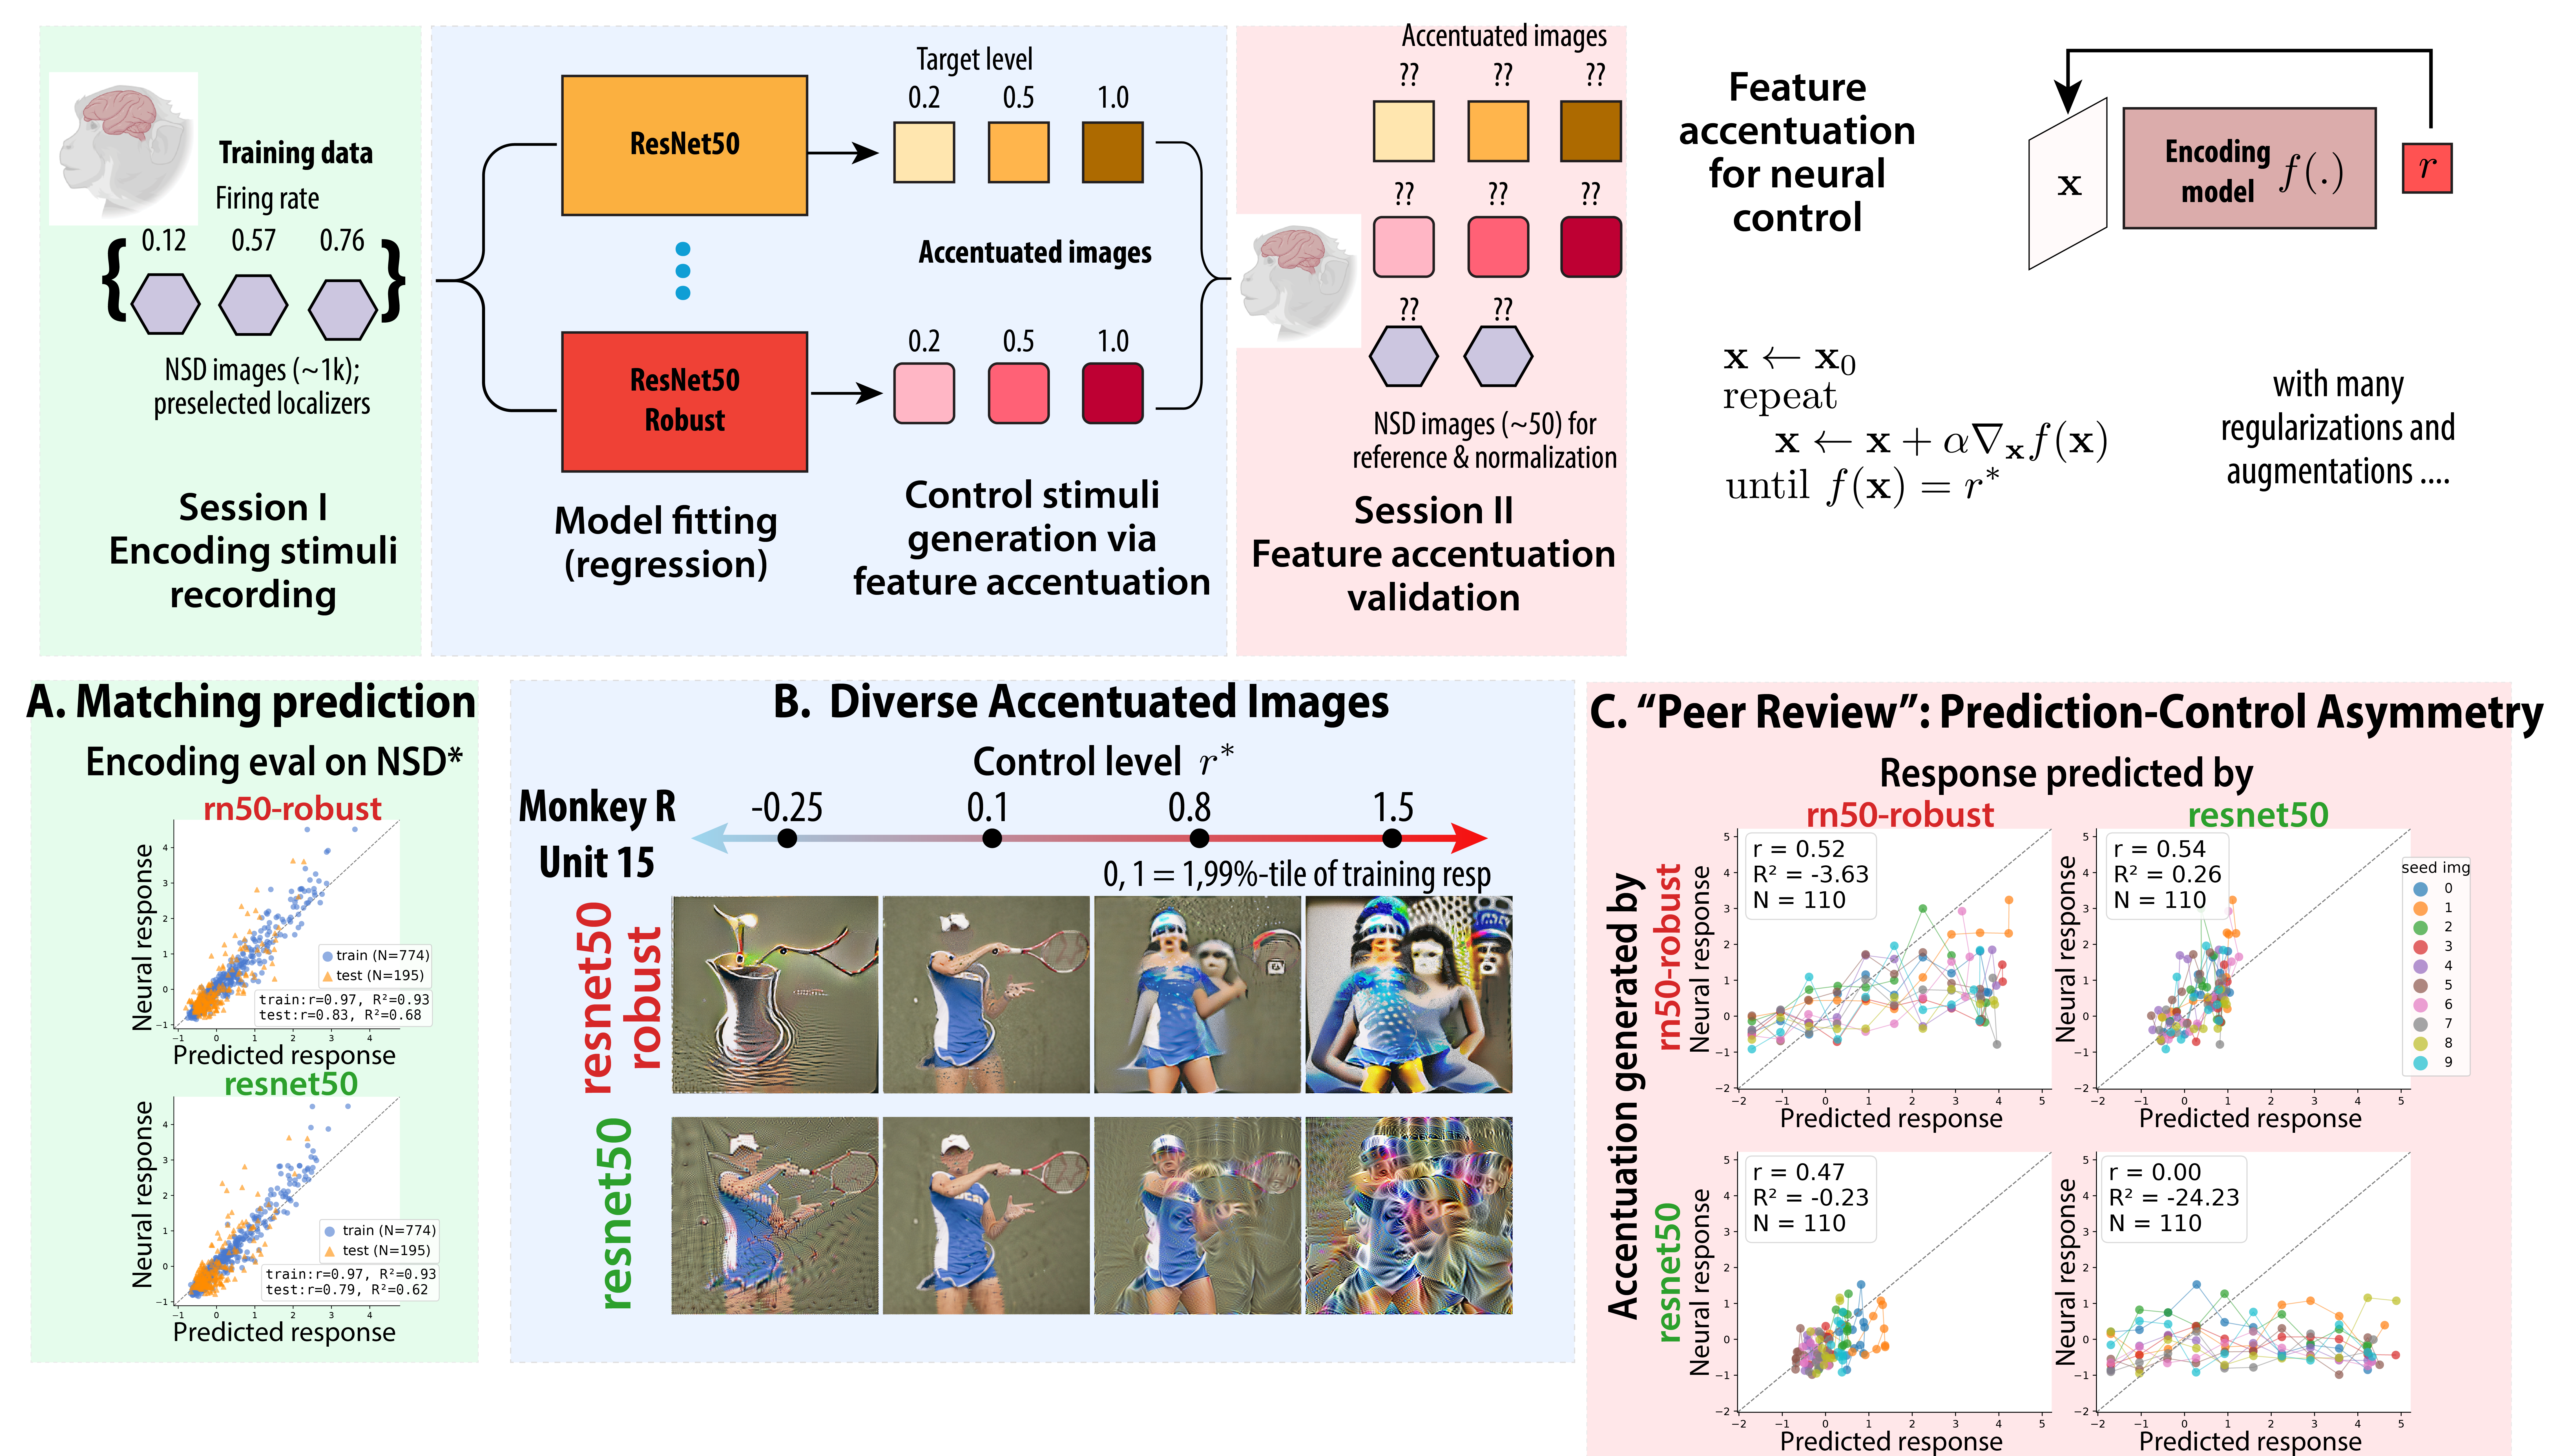
\includegraphics[width=\linewidth]{figures/Figure_NeuroCtrl_results.png}\\[2pt]
    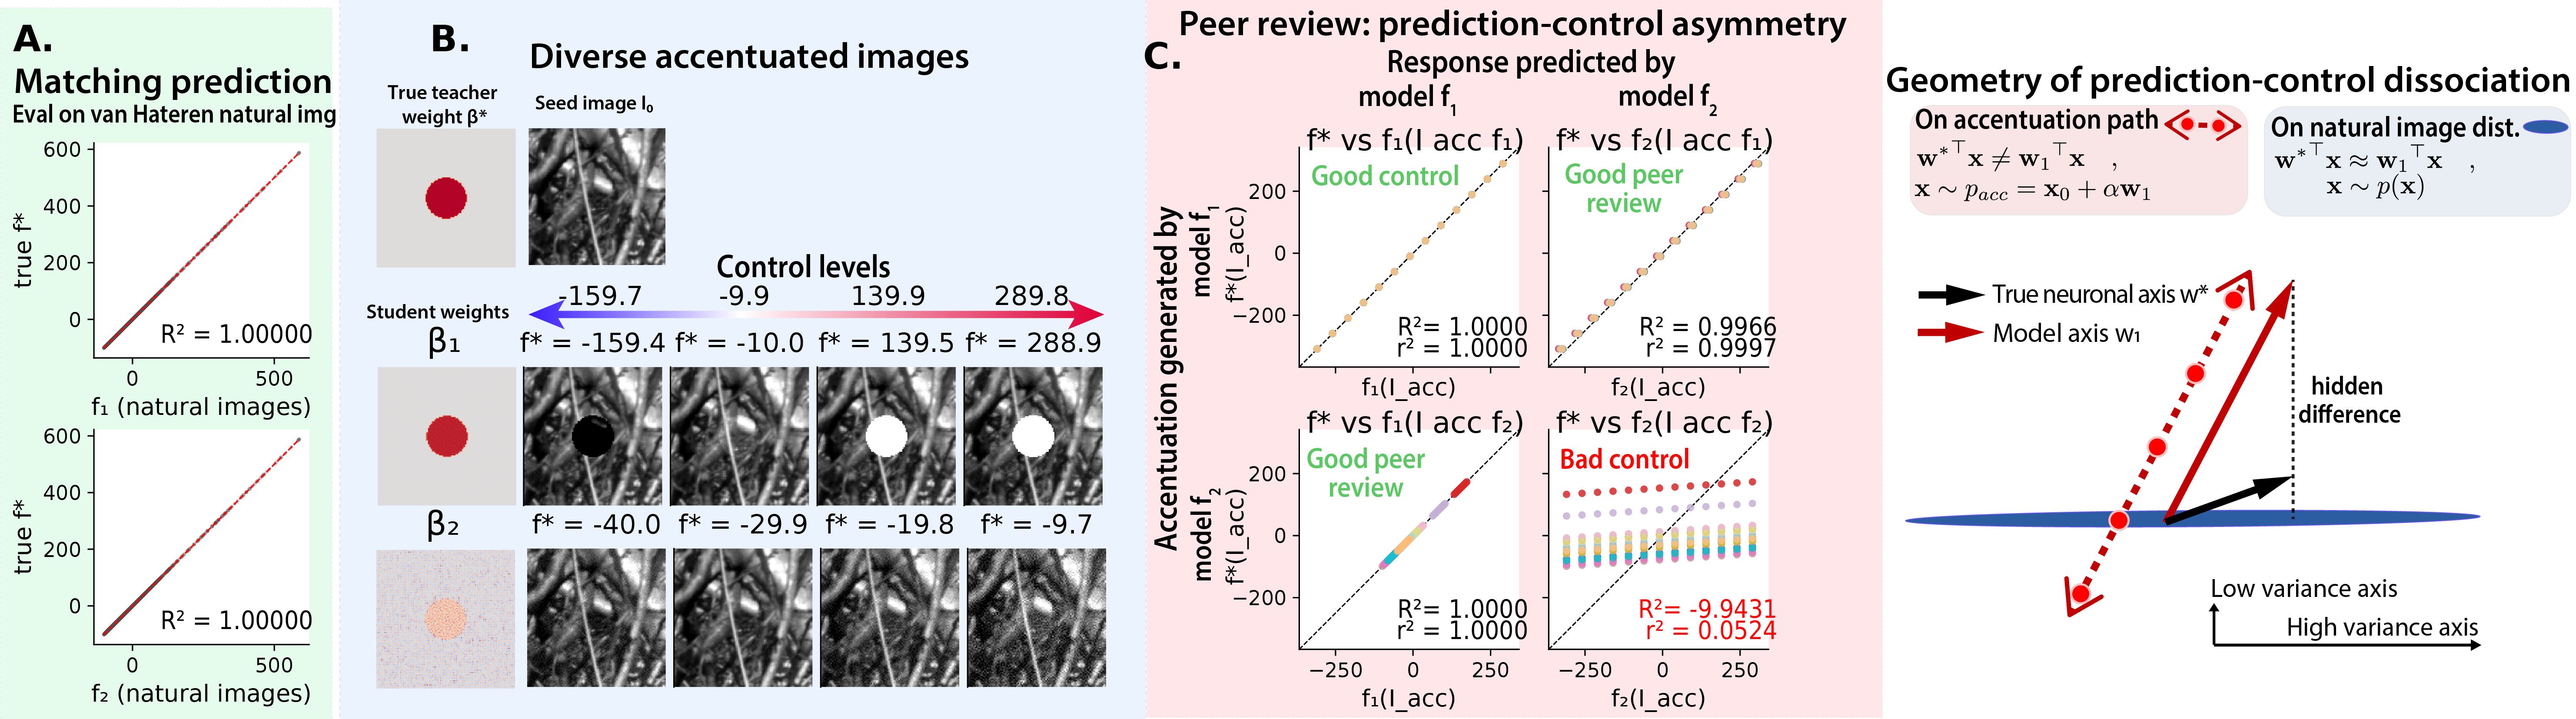
\includegraphics[width=\linewidth]{figures/Figure_LinearToyModel-04.png}
    \caption{\textbf{The same three phenomena in neurons (top) and in a linear teacher--student model (bottom).}
    Top: closed-loop experiment of \citetPW. Encoding models are fit to responses to natural images, generate accentuated images for graded target responses, and are tested in a second session.
    \textbf{A}~Two models predict held-out natural-image responses equally well.
    \textbf{B}~Their accentuations from the same seed differ visibly, and only one modulates the neuron.
    \textbf{C}~Peer review: each model evaluated on the other's images. The weak controller tracks the strong controller's images but its own images barely modulate the neuron.
    Bottom: two linear students of a linear teacher (a disk-shaped weight on van~Hateren images), differing only along low-variance image directions, reproduce A--C exactly. Geometry inset: prediction sees weight error through the covariance ellipse; the accentuation path exposes the hidden Euclidean difference. Details: App.~\ref{sec:app-methods-neural-data} (neurons), App.~\ref{sec:app-methods-toy} (linear model).}
    \label{fig:phenomena}
\end{figure}


\citetPW   used the following closed-loop paradigm (Fig.~\ref{fig:phenomena}, top): responses of visual cortical sites (V2--IT, 25 sites in 5 macaques) to $\sim$1000 natural images were recorded; for each site, ten encoding models were fit by ridge regression on features from ten deep network backbones, with penalty and layer chosen by cross-validation; using \emph{feature accentuation} \citep{hamblin2024feature}, each model optimized a image using a variant of gradient ascent, and then synthesized images that drive its own prediction to eleven target levels from ten seed images (Fig.~\ref{fig:phenomena}, top right); and the images were presented to the same sites in the \textit{control session}. The control is successful if the proposed images evoked neural activations as predicted (data and models: Apps.~\ref{sec:app-methods-neural-data},~\ref{sec:app-methods-models}). Three observations motivate this paper.

\paragraph{Similar prediction, divergent control.}
The trained models were tightly matched on held-out natural images (Fig.~\ref{fig:phenomena}\red{A}), yet the slope and correlation between predicted and measured responses to their own accentuated images varied widely across models, with far larger spread than on natural images. Many models reached their target \emph{predicted} response by adding texture and high-spatial-frequency structure that left the neuron largely unmoved (Fig.~\ref{fig:phenomena}\red{B,C}).

\paragraph{Recognition without generation.}
Presenting model A's images to model B (``peer review'', Fig.~\ref{fig:phenomena}\red{C}) shows an asymmetry: a model whose own images fail to modulate the neuron still predicts the neuronal responses to a successful model's images with good correlation and better $R^2$ than the generator itself. Models can recognize good control stimuli that they cannot produce.

\paragraph{Control tracks input-gradient structure.}
Across the 250 site--model pairs, control success is predicted by the spectral profile of the model's input gradient $\nabla_\x f$: models whose gradients concentrate power at low spatial frequencies, like natural images, control better. The two adversarially trained models are the strongest controllers, but the association persists without them.

These phenomena are puzzling at first glance, but linear models on natural images reproduce all three observations (Fig.~\ref{fig:phenomena}, bottom). We construct the bad controller to differ from the teacher along the lowest-variance, high-spatial-frequency directions of the image covariance, the good controller only slightly and along less extreme ones; then matched prediction, diverse accentuations, unequal control and good peer review all follow. Dissecting this idealistic set up, the rest of the paper explains why \textit{finite-sample} regression on \textit{noisy responses} produces such errors, why \textit{cross-validation does not remove them}, and how \textit{feature maps} can amplify the dissociation. 

% These phenomena are puzzling at first glance, though we show, linear models on natural images can reproduce all three observations (\red{
% bottom, Fig.~\ref{fig:phenomena}}). 
% We constructed the bad controller to have weight error along low-variance directions of the image covariance (high spatial frequency), while the good controller has weight error more along the high eigenspace. Then matched prediction on natural data; diverse generated images; unequal control outcomes and relatively good peer reviews all emerge from it. 
% This shows the same symptom can emerge without deep network, nonlinearity or neurons. 
% Dissecting this idealistic set up, the remainder of the paper explains why \textit{finite-sample} regression on \textit{noisy responses} produces this failure, why \textit{cross-validation does not eliminate it}, and how \textit{feature maps} introduce additional degrees of freedom that can greatly amplify the prediction--control dissociation. 



\section{Three evaluations, three geometries of one predictor}
\label{sec:setup}

\paragraph{Teacher and student.}
We idealize a visual neuron as a noisy linear teacher, its encoding model as a linear student, and natural image inputs as $\x\in\R^d,\x\sim\mathcal N(0,\Sigma)$, a centered Gaussian distribution with structured covariance $\Sigma=\sum_ks_k\uvec_k\uvec_k^\top$. 
A linear teacher with weight $\bstar=\sum_kb_k\uvec_k$ produces noisy responses $y=\x^\top\bstar+\sigma\epsilon$, $\epsilon\sim\mathcal{N}(0,1)$, and $S:={\bstar}^\top\Sigma\bstar$ is the noiseless natural response variance. 
The student is $f(\x)=\x^\top\bhat$, fitted from $n$ pairs $(X,\mathbf y)$; for linear feature-space students (Sec.~\ref{sec:feature}) $\bhat$ is the effective pixel weight $F^\top\hat w$, which is also the gradient $\nabla_\x f$.

\paragraph{Three distributions.}
Generalization evaluates $f$ on fresh natural inputs, $\x\sim\mathcal N(0,\Sigma)$. Accentuation evaluates $f$ on inputs it generates itself: gradient ascent from a seed $\x_0$ moves along $\nabla_\x f=\bhat$, so the idealized path is $\x=\x_0+\alpha\bhat$ with $\alpha$ set by the target level\footnotemark. %In the main text, 
We study $\x_0=0$ and the target range is variance-matched, $\Var[\alpha]({\bhat}^\top\bhat)^2=S$, so the student's \emph{prediction} has natural dynamic range along its path. Peer review evaluates $f$ on the path $\x_0+\alpha\bprime$ generated by another student $\bprime$. Writing $\Delta=\bhat-\bstar$ and applying the standard formulas for MSE, $R^2$ and the slope of true-on-predicted response to each distribution (Lem.~\ref{lem:mr-metrics}) gives Table~\ref{tab:evaluation-metrics}.
\footnotetext{In practice, accentuation for DNN adds gradient preconditioning and augmentation \citep{hamblin2024feature,MACO}, some supplied image priors \cite{XXX}; App.~\ref{sec:app-evaluation-distributions} treats nonzero and multiple seeds.}

\begin{table}[t]
\vspace{-10pt}
\centering\footnotesize\setlength{\tabcolsep}{3.5pt}
\resizebox{\ifdim\width>\linewidth\linewidth\else\width\fi}{!}{%
\begin{tabular}{@{}llcccl@{}}
\toprule
Evaluation & Covariance & MSE $E$ & $R^2$ & Slope & Equal-error set \\
\midrule
Generalization & $\Sigma$ & $\Delta^\top\Sigma\Delta$ & $1-\Delta^\top\Sigma\Delta/S$ & ${\bhat}^\top\Sigma\bstar/{\bhat}^\top\Sigma\bhat$ & ellipsoid \\
Accentuation & $\Var[\alpha]\,\bhat{\bhat}^\top$ & $S\,(1-N/D)^2$ & $1-(D/N-1)^2$ & $N/D$ & sphere \\
Peer review & $\Var[\alpha']\,\bprime{\bprime}^\top$ & $S\,(D_{peer}-N_{peer})^2/\|\bprime\|^4$ & $1-(D_{peer}/N_{peer}-1)^2$ & $N_{peer}/D_{peer}$ & hyperplane \\
\bottomrule
\end{tabular}}
\caption{Evaluation metrics on three distributions, and their geometries. $\Delta:=\bhat-\bstar$; on the student's own path the true and predicted gains are $N:={\bhat}^\top\bstar$, $D:={\bhat}^\top\bhat$, and on a peer's path $N_{peer}:={\bstar}^\top\bprime$, $D_{peer}:={\bhat}^\top\bprime$; $z:=D/N-1$ in each row. Last column: level sets of each row's metrics in the space of student weights $\bhat$ (Prop.~\ref{prop:mr-iso-geometry}).}
% \caption{One fitted weight, three evaluation distributions, three geometries. $\Delta:=\bhat-\bstar$; on the student's own path the true and predicted gains are $N:={\bhat}^\top\bstar$, $D:={\bhat}^\top\bhat$, and on a peer's path $N_{peer}:={\bstar}^\top\bprime$, $D_{peer}:={\bhat}^\top\bprime$; $z:=D/N-1$ in each row. The last column is the level set of each row's metrics in the space of student weights $\bhat$: an ellipsoid about $\bstar$, a sphere on the diameter $[0,(1+z)\bstar]$, a hyperplane normal to $\bprime$ (Prop.~\ref{prop:mr-iso-geometry}). Pearson correlation is degenerate on a noiseless rank-one path and is omitted.}
\label{tab:evaluation-metrics}
\vspace{-17pt}
\end{table}

\paragraph{Prediction is covariance-weighted, control is Euclidean.}
Generalization error is $E_{gen}=\Delta^\top\Sigma\Delta$: a weight error $\Delta$ along $\uvec_k$ costs $s_k$ times its squared length, so errors in low-variance directions can be nearly invisible. For accentuation, weight error is evaluated on a single path $\bhat$, and every metric is a function of the scalar $z$, or equivalently the ratio between quadratic forms $D/N$, 
\begin{equation}\small
z_{acc}:=\frac DN-1=\frac{{\bhat}^\top(\bhat-\bstar)}{{\bhat}^\top\bstar},
\qquad
\frac{E_{acc}}{S}=\Big(\frac{z}{1+z}\Big)^2,\quad R^2_{acc}=1-z^2,\quad \mathrm{slope}_{acc}=\frac{1}{1+z},
\label{eq:acc_metric_ND_depen}
\end{equation}
\begin{wrapfigure}[26]{r}{0.45\linewidth}
    \vspace{-8pt}
    \centering
    \vspace{-5pt}
    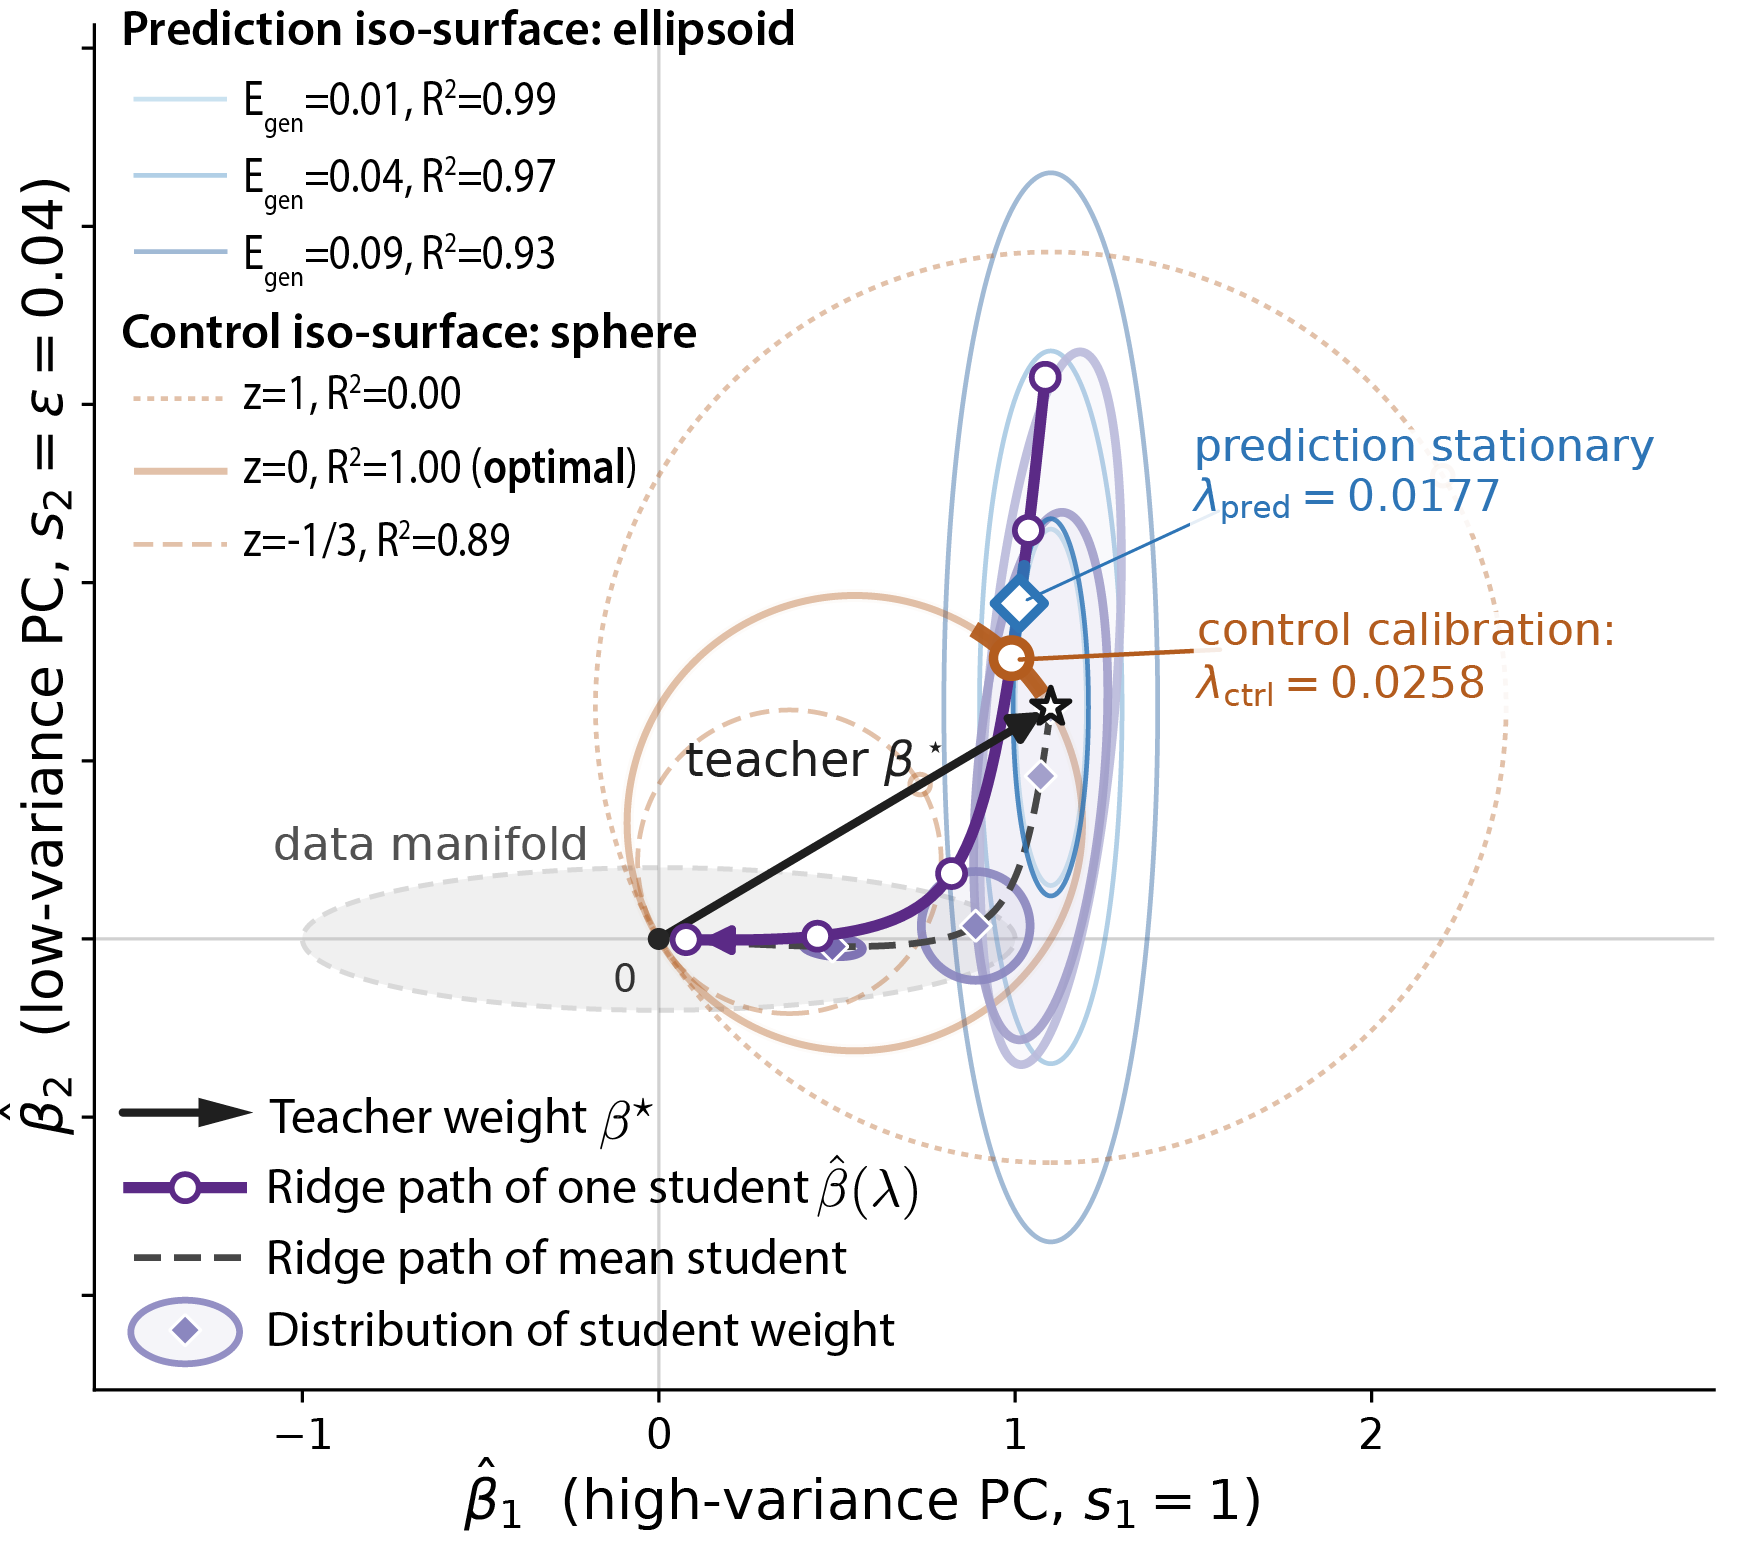
\includegraphics[width=\linewidth]{figures/Figure_iso_err_surf_dissociation-01.png}
    \vspace{-20pt}
    \caption{\textbf{Equal-error sets and the ridge path} in the plane of a high- and a low-variance PC. Prediction levels are ellipsoids around $\bstar$ (blue), control levels are the spheres with diameter joining $0$ and $(1+z)\bstar$ (orange). The fitted weight traverses this plane as a function of $\lambda$ (purple), scattering around the mean Ridge path (dashed black). Cross-validation picks the tangency of the path with an ellipsoid; perfect control is its crossing with the $z=0$ sphere. Exact two-dimensional construction: App.~\ref{sec:app-ext-geometry}. }
    \label{fig:geometry}
\end{wrapfigure}
The three evaluations therefore have three geometries in the space of student weights (Table~\ref{tab:evaluation-metrics}, last column; Prop.~\ref{prop:mr-iso-geometry}; Fig.~\ref{fig:geometry}).
\textbf{Prediction: ellipsoids.} The equal-$E_{gen}$ sets are ellipsoids centered on $\bstar$ with semi-axis $\sqrt{E_{gen}/s_k}$ along $\uvec_k$, hence elongated along low-variance axes, where large weight errors are cheap.
\textbf{Control: spheres.} The equal-$z_{acc}$ sets are Euclidean spheres whose diameter joins $0$ and $(1+z)\bstar$; the diameter encodes the error directly, and zero-error students live on the sphere through $\bstar$ at $z=0$, not only at $\bstar$ itself.
\textbf{Peer review: hyperplanes.} The equal-$z_{peer}$ sets are hyperplanes normal to the generator $\bprime$, so a peer reviewer is judged only on its component along the peer's path.
A student can sit deep inside a small prediction ellipsoid, lie on a huge control sphere, and still lie on the zero-error hyperplane of a good generator: this is exactly the configuration of Fig.~\ref{fig:phenomena} (bottom), and it can be made arbitrarily extreme by adding weight along a direction with $s_k\to0$ (Ex.~\ref{ex:mr-dissociation}).


The remaining question is therefore not whether the dissociation is possible but when \emph{learning} produces it. We study three ingredients: finite-sample regression on noisy responses, the choice of regularization, and the feature map through which the gradient reaches the pixels. % We take them in turn.

\section{Pixel-space ridge: noise, spectrum and regularization}
\label{sec:pixel}

Ridge regression in pixel space, $\bhat=\arg\min_\beta\frac1n\|X\beta-\mathbf y\|^2+\lambda\|\beta\|^2$, yields
\begin{equation}
\bhat=\underbrace{(\hat\Sigma+\lambda I)^{-1}\hat\Sigma\bstar}_{\text{mean: signal shrinkage}}
+\underbrace{\sigma(\hat\Sigma+\lambda I)^{-1}\tfrac1nX^\top\eta}_{\text{noise}},
\qquad \hat\Sigma=X^\top X/n,
\quad
\mathbf y=X\bstar+\sigma \eta
\label{eq:ridge}
\end{equation}
Ridge penalizes weight in low-variance directions, so one might expect it to remove these control-vulnerable components; we ask whether they survive a cross-validated penalty.

\paragraph{The ridge path through the two landscapes.}
The question has a geometric reading (Fig.~\ref{fig:geometry}). For a given training set, Eq.~\ref{eq:ridge} traces a path $\bhat(\lambda)$ in weight space from the least-squares or minimum-norm solution at $\lambda\to0$ to the origin at $\lambda\to\infty$. Response noise and the random design scatter the fitted weight in a cloud around its mean. Ideally, cross-validation selects the point where the path is tangent to the smallest reachable prediction ellipsoid; whereas minimal control error asks where the path crosses the $z=0$ sphere $D=N$; in general the two points differ, and the analysis below makes this quantitative. 
%\red{the two coincide only if the noise cloud has not pushed the path off the sphere in the directions the ellipsoid does not see. The deterministic equivalents below compute where the center of this cloud sits, how much Euclidean spread it carries, and hence the distance between the two points.}, and the cloud is elongated along the low-variance directions of $\Sigma$, because those are the directions the data constrain least


\paragraph{Toolkit.}
We use deterministic equivalents (DEs) in the proportional limit $d/n\to\gamma$ \citep{dobriban2018high,hastie2022surprises}. They replace functions of the empirical covariance $\hat\Sigma$ by deterministic functions of the population covariance $\Sigma$, e.g. $\hat\Sigma(\hat\Sigma+\lambda I)^{-1}\asymp\Sigma(\Sigma+\kappa I)^{-1}$, where the finite-sample randomness is absorbed into an effective penalty $\kappa(\lambda)\ge\lambda$, the unique positive root of $\kappa-\lambda=\frac{\kappa}{n}\operatorname{Tr}[\Sigma(\Sigma+\kappa I)^{-1}]$, one-to-one in $\lambda$ (App.~\ref{sec:app-de-toolkit}).
Applied to Eq.~\ref{eq:ridge}, the DE says that the signal term concentrates around a \emph{mean fitted weight}, the teacher shrunk mode by mode,
\begin{equation}
\bar\beta_\kappa:=\Sigma(\Sigma+\kappa I)^{-1}\bstar=\sum_k\frac{s_k}{s_k+\kappa}\,b_k\uvec_k ,
\label{eq:pixel-mean-weight}
\end{equation}
while the noise term has zero mean but carries Euclidean energy, the \emph{norm inflation} $V:=\E\|\bhat\|^2-\|\bar\beta\|^2\ge0$, which drives accentuation error. The mean weight $\bar\beta$ and inflation $V$ also organize the feature-space case and the nonlinear diagnostic (Secs.~\ref{sec:feature},~\ref{sec:nonlinear}). Results use the teacher-weighted and unweighted spectral sums
\begin{equation}\small 
B_{p,q}(\kappa)=\sum_k\frac{s_k^p}{(s_k+\kappa)^q}b_k^2,\qquad
\mathrm{df}_{p,q}(\kappa)=\sum_k\frac{s_k^p}{(s_k+\kappa)^q},\qquad \mathrm{df}_2:=\mathrm{df}_{2,2},
\end{equation}
so that, for instance, $\bstar^\top\bar\beta_\kappa=B_{1,1}$ and $\|\bar\beta_\kappa\|^2=B_{2,2}$. 
For the ratio $N/D$ we use the leading approximation $\mu_N/\mu_D$ from the DEs of $N$ and $D$; second-order and distributional refinements matter only where the leading calibration error is already small (App.~\ref{sec:app-ratio-corrections}).

\begin{figure}[t]
    \centering
    \vspace{-19pt}
    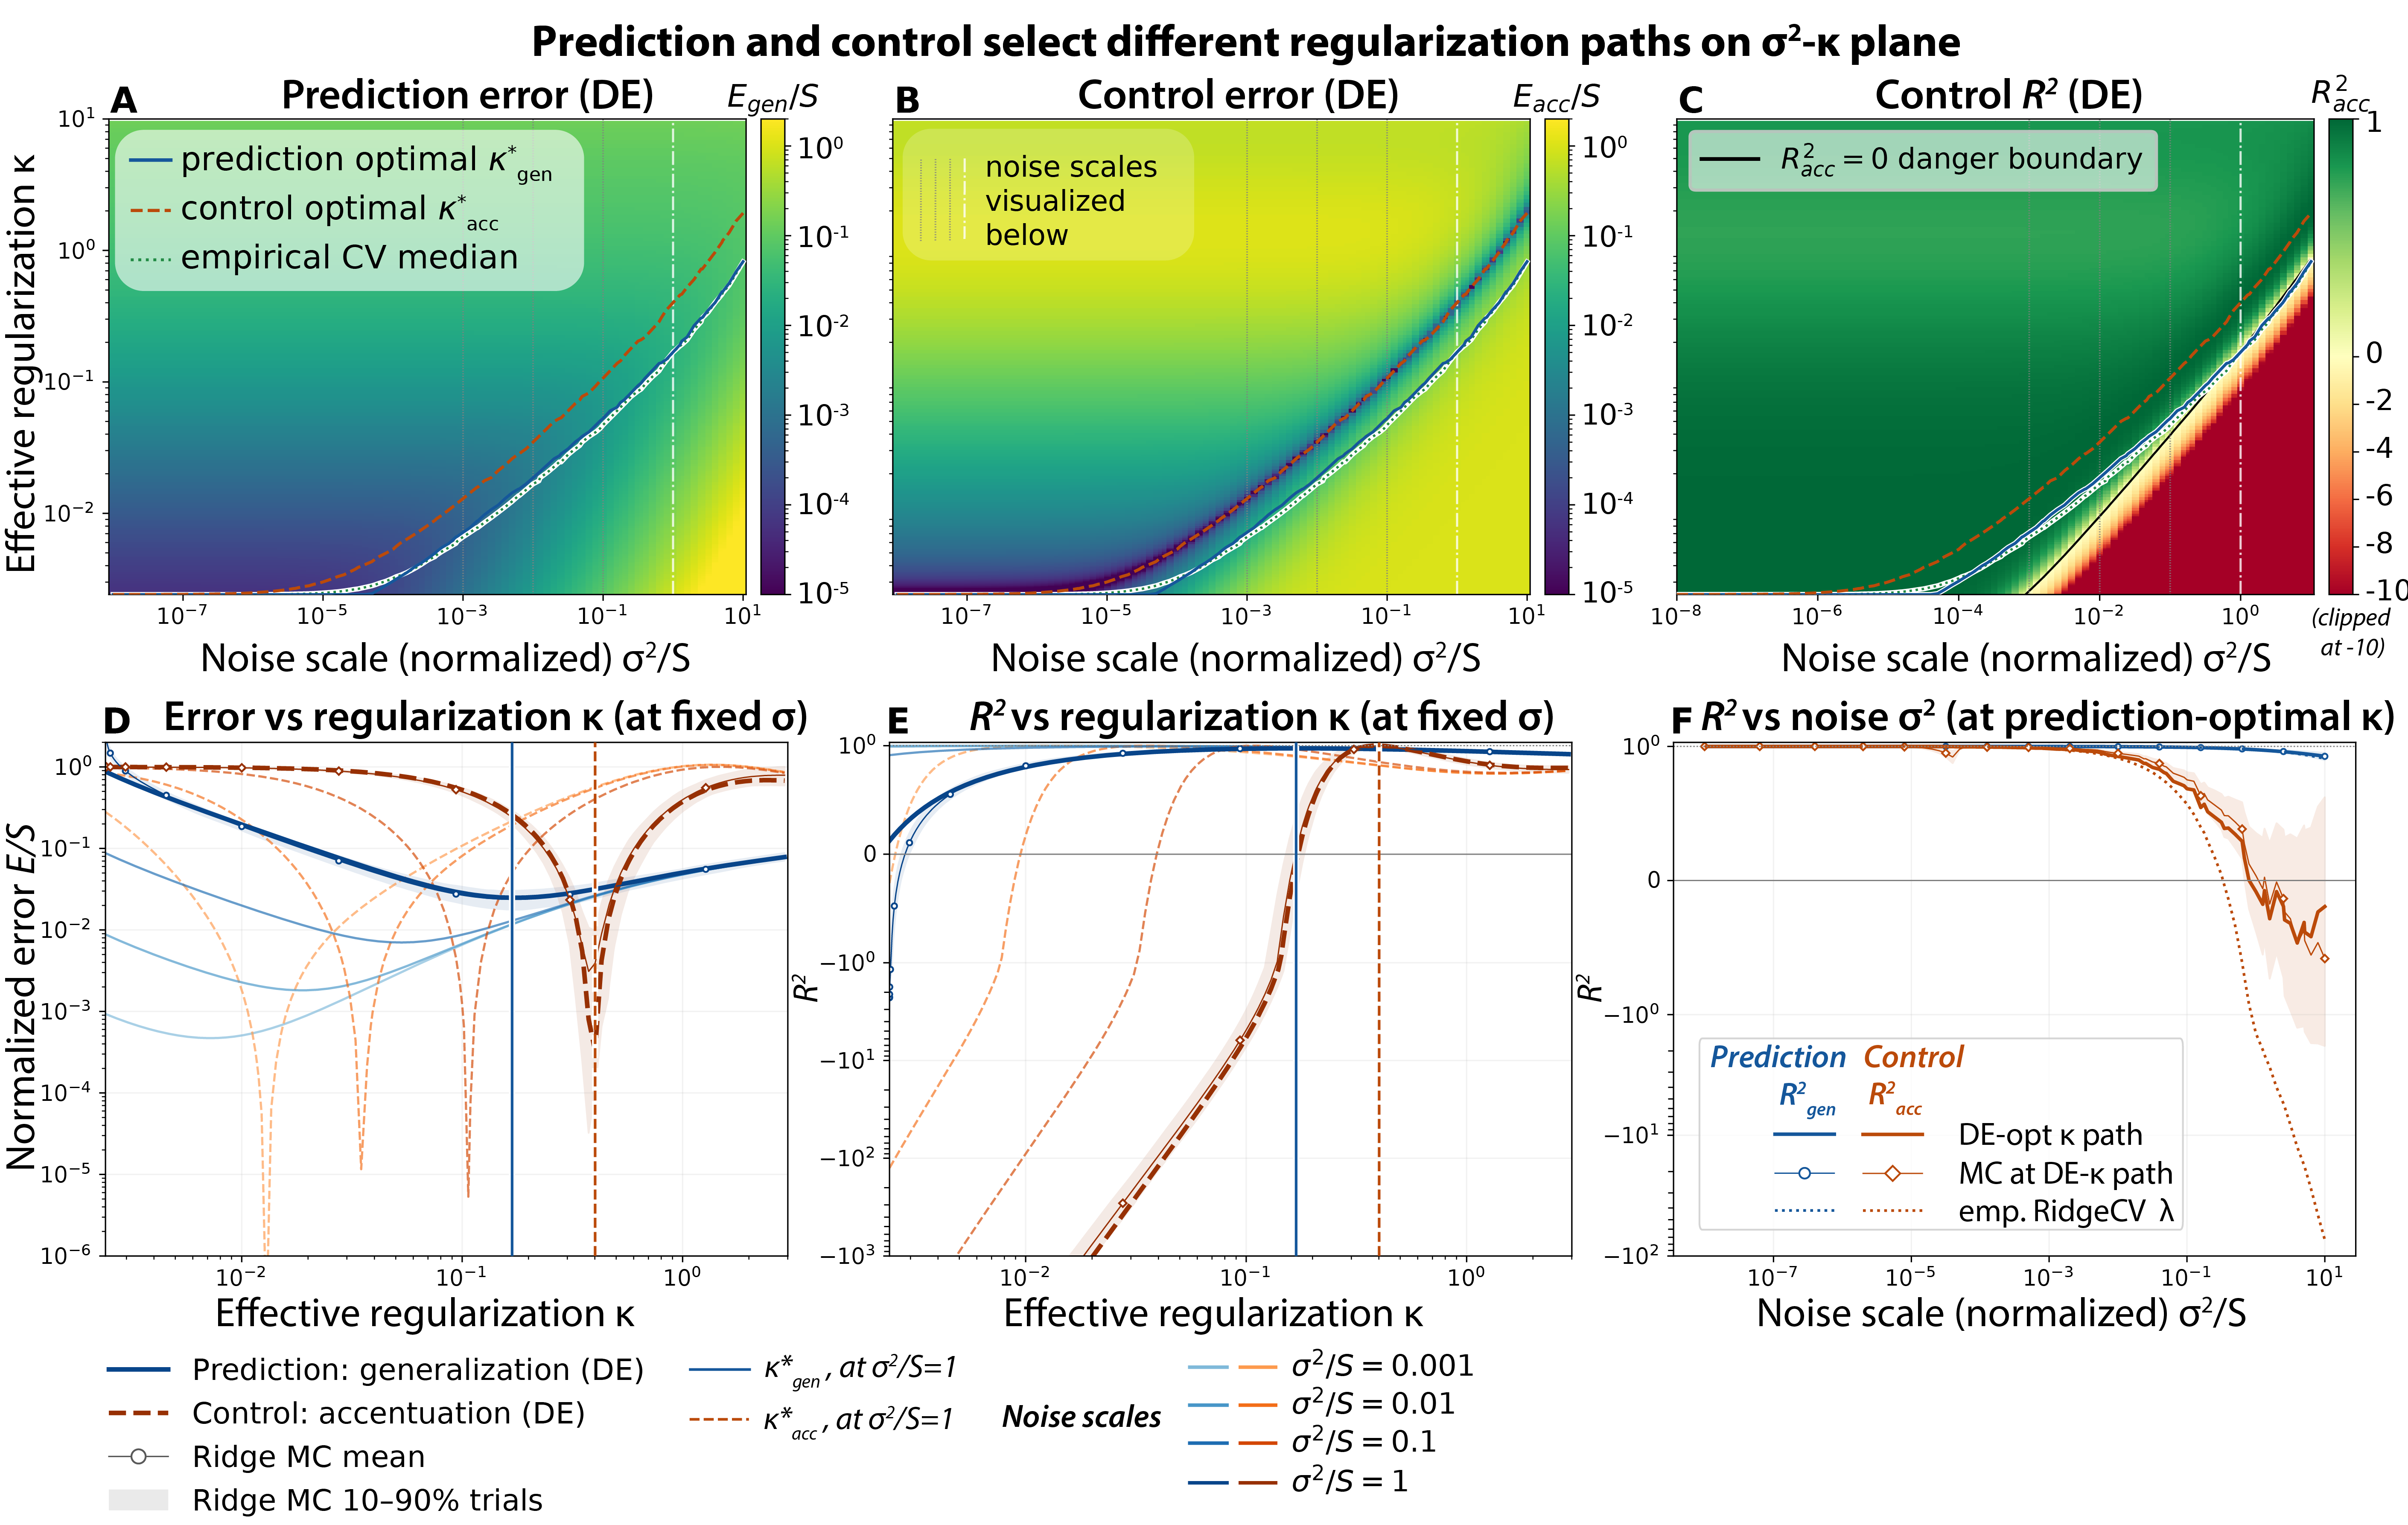
\includegraphics[width=\linewidth]{figures/Figure_PixRidgeGeometry.png}
    \vspace{-15pt}
    \caption{\textbf{Pixel-space ridge separates prediction- and control-optimal regularization on natural images.}
    Disk teacher on van~Hateren images ($d=10^4$, $n=10^3$).
    \textbf{A--C}~DE landscapes (Eq.~\ref{eq:pixel-de}) of $E_{gen}$, $E_{acc}$ and $R^2_{acc}$ over noise $\sigma^2/S$ and effective penalty $\kappa$ (Monte Carlo: Fig.~\ref{fig:supp-pixel-de-mc}). The prediction-optimal and median empirical RidgeCV paths track each other but not the control-optimal path; black contour: $R^2_{acc}=0$. 
    \textbf{D,E}~Slices at four noise levels expose displaced prediction and control valleys (or peaks for $R^2$); markers and bands show the mean and 10--90\% range over 100 natural-image trials at the highlighted noise $\sigma^2/S=1$.
    \textbf{F}~Along the prediction-optimal path, $R^2_{gen}$ remains high while $R^2_{acc}$ becomes strongly negative; empirical RidgeCV exhibits the same dissociation. Methods: App.~\ref{sec:app-vanhateren-landscape-methods}; further views: App.~\ref{sec:app-ext-pixel}.}
    \vspace{-15pt}
    \label{fig:pixel}
\end{figure}

\begin{prop}[Pixel ridge: prediction and control]\label{prop:pixel-de}
With $\kappa$, $B$ and $\mathrm{df}$ built from $\Sigma$,
\begin{equation}
\begin{aligned}
E_{gen}&\asymp E_{gen,DE}=\frac{n(\kappa^2B_{1,2}+\sigma^2)}{n-\mathrm{df}_2}-\sigma^2,\qquad
N\asymp \mu_N=\bstar^\top\bar\beta_\kappa=B_{1,1},\\
D&\asymp \mu_D=\|\bar\beta_\kappa\|^2+V_{\rm pix}(\kappa),
\qquad
V_{\rm pix}(\kappa)=\frac{\mathrm{df}_{1,2}(\kappa)}{n}\big(E_{gen,DE}+\sigma^2\big).
\end{aligned}
\label{eq:pixel-de}
\end{equation}
(Proofs and the per-mode decomposition behind these sums: App.~\ref{sec:app-pixel-ridge}.)
\end{prop}
$E_{gen}$ recovers the classical in-distribution generalization error \citep{dobriban2018high,hastie2022surprises}. $N$ is the alignment of the teacher with the mean fitted weight, and the first term of $D$ is that weight's squared norm; both are set by the teacher and the shrinkage alone, and since each factor $s_k/(s_k+\kappa)$ lies in $[0,1]$ they are ordered $\|\bstar\|^2\ge B_{1,1}\ge B_{2,2}$ (Eq.~\ref{eq:app-spectral-inequalities}), so the mean weight by itself \emph{under}-shoots its own path ($D<N$, slope above one). The second term, $V_{\rm pix}$, is how limited data $n$, response noise $\sigma^2$ and prediction error $E_{gen}$ jointly inflate the student norm, amplified by the spectral susceptibility $\mathrm{df}_{1,2}=\sum_ks_k/(s_k+\kappa)^2$, which counts the modes near the threshold $\kappa$. 
Inflation enlarges $D$ without changing $N$, so the student can easily \emph{over}-predict: $\mathrm{slope}_{acc}=N/D$ drops below one, and $z=D/N-1$ can grow until $R^2_{acc}=1-z^2$ turns negative.
Note that $V$ is not necessarily bad for control: at the special point $B_{1,1}=B_{2,2}+V_{\rm pix}$ the inflation exactly replenishes the norm lost to shrinkage, so $N=D$ and control is perfect at leading order (the valley in Fig.~\ref{fig:pixel}\textbf{B}).
This is generally not where cross-validation lands, as the next proposition shows.
%that, for a natural-image spectrum, accumulates over thousands of weakly constrained high-frequency modes

\begin{prop}[Prediction-optimal and control-optimal penalties differ]\label{prop:pixel-tuning}
Among admissible values of $\kappa$, let $\kappa_{\rm gen}^{\star}$ be an
interior differentiable minimizer of $E_{\rm gen,DE}$, and let
$\kappa_{\rm acc}^{\star}$ denote a zero of the leading control error,
equivalently satisfying $\mu_D=\mu_N$. Their defining conditions are
\begin{align}
E_{\rm gen,DE}+\sigma^2
&=n\kappa\frac{B_{2,3}}{\mathrm{df}_{2,3}},
&&(\kappa=\kappa_{\rm gen}^{\star};\ \text{prediction stationarity}),
\label{eq:gen_optim_reg_cond}\\
E_{\rm gen,DE}+\sigma^2
&=n\kappa\frac{B_{1,2}}{\mathrm{df}_{1,2}},
&&(\kappa=\kappa_{\rm acc}^{\star};\ \text{zero leading control error}).
\label{eq:acc_optim_reg_cond1}
\end{align}
% An interior minimizer of $E_{gen,DE}$ and a zero of the leading control error satisfy, respectively,
% \begin{equation}
% E_{gen,DE}+\sigma^2=n\kappa\frac{B_{2,3}}{\mathrm{df}_{2,3}}
% \quad\text{(prediction)},\qquad
% E_{gen,DE}+\sigma^2=n\kappa\frac{B_{1,2}}{\mathrm{df}_{1,2}}
% \quad\text{(control)},
% \label{eq:acc_optim_reg_cond1}
% \end{equation}
Further, at the prediction optimum $\kappa_{\rm gen}^{\star}$ the control error is
\begin{equation}
z^{(0)}_{acc,CV}=\frac{\kappa\,\mathrm{df}_{1,2}}{B_{1,1}}
\left(\frac{B_{2,3}}{\mathrm{df}_{2,3}}-\frac{B_{1,2}}{\mathrm{df}_{1,2}}\right)_{\kappa=\kappa^\star_{gen}} .
\label{eq:pixel-zacc-cv}
\end{equation}
(Proofs: App.~\ref{sec:app-optimal-regularization}.)
\end{prop}
Geometrically, along the ridge path (Fig.~\ref{fig:geometry}), $\kappa_{\rm gen}^{\star}$ lands at the tangency with the prediction ellipsoid and $\kappa_{\rm acc}^{\star}$ at its crossing of the control sphere. 
Both conditions equate the noisy prediction risk to $n\kappa$ times a spectral-band average of the teacher's per-mode power $b_k^2$, but the two bands sit at different places (App.~Fig.~\ref{fig:app-tuning-kernels}). The control kernel $s_k/(s_k+\kappa)^2$ is a bump centered at $s_k=\kappa$, symmetric on a log axis; the prediction kernel $s_k^2/(s_k+\kappa)^3$ is the same bump multiplied by the shrinkage factor $s_k/(s_k+\kappa)$, which shifts it up to $s_k\approx2\kappa$ and suppresses its low-variance side. 
% \red{Each kernel is a $\kappa$-sensitivity: the control condition asks which modes' shrinkage $s_k/(s_k+\kappa)$ changes as $\kappa$ moves, since that sets the mean weight $\bar\beta_\kappa$ and $N$, whereas prediction stationarity asks which modes' \emph{squared} shrinkage changes, since that sets $E_{gen}$.} 
Consequently $z^{(0)}_{acc,CV}$ compares the teacher power around $2\kappa$ with that around $\kappa$. 
It vanishes for isotropic data, or for a teacher whose per-mode power $b_k^2$ is constant across modes (\red{Rem.~\ref{rem:app-tuning-remarks}}). 
For \textit{an anisotropic spectrum and a structured teacher} the averages differ, and their difference is the control error left at the cross-validated penalty. When $b_k^2$ decreases toward the low-variance tail, as for a teacher aligned with high-variance image modes, $z^{(0)}_{acc,CV}>0$ and the cross-validated student over-predicts ($\mathrm{slope}_{acc}<1$). 
% ; and it is negative in the opposite case.
 %teacher-weighted spectral average $B_{,}$, but they average with different powers of $s_k/(s_k+\kappa)$. 
% Eq.~\ref{eq:pixel-zacc-cv} is the distance along the path between its tangency with the prediction ellipsoid and its crossing of the control sphere.
%The gap is multiplied by $\kappa\,\mathrm{df}_{1,2}$, i.e. by the number of modes near the regularization edge. 

Over the noise--regularization plane for natural images (Fig.~\ref{fig:pixel}A--C), the DE tracks Monte Carlo except at very low noise or regularization (Fig.~\ref{fig:supp-pixel-de-mc}). Prediction- and control-optimal penalties form two distinct valleys, the $E_{acc}$ valley a sharp cusp. At low noise $\kappa^\star_{\rm gen}$ is also benign to control; as noise grows it approaches and crosses the $R^2_{acc}=0$ cliff, and control fails catastrophically. 

% Figure~\ref{fig:pixel} confirms the picture on real natural-image regression. The DE surfaces track Monte Carlo over eight decades of noise; the prediction-optimal and control-calibrated penalties form two distinct ridges; and along the cross-validated path the student remains an excellent predictor while its accentuation $R^2$ becomes negative at moderate noise. 

% \red{In Fig.~\ref{fig:geometry}, Eq.~\ref{eq:pixel-zacc-cv} is the distance along the path between its tangency with the prediction ellipsoid and its crossing of the control sphere.} 
For pixel regression, then, \emph{control is bad despite prediction-optimal regularization when the response is noisy, the spectrum anisotropic and many modes sit near $\kappa$}: the regime of noisy neurons viewing natural images. 



\paragraph{Peer review: recognition without generation.}
Peer review evaluates $\bhat$ on the path of a peer $\bprime$, so the roles of $N$ and $D$ are played by the true and predicted gains along the peer's path, $N_{peer}={\bstar}^\top\bprime$ and $D_{peer}={\bhat}^\top\bprime$ of Table~\ref{tab:evaluation-metrics}. Take the peer to be a ridge fit at the same $\kappa$ on independent data. Both fits then concentrate around the same mean weight $\bar\beta_\kappa$ while their noise parts are uncorrelated, so the norm inflation drops out of the cross product: $D_{peer}\asymp\|\bar\beta_\kappa\|^2=B_{2,2}$ and $N_{peer}\asymp\bstar^\top\bar\beta_\kappa=B_{1,1}$ (Prop.~\ref{prop:mr-peer}). The peer slope and score are therefore
\begin{equation}
\mathrm{slope}_{peer}=\frac{N_{peer}}{D_{peer}}\asymp\frac{B_{1,1}}{B_{2,2}}\in[1,\infty),
\qquad
R^{2,(0)}_{peer}=1-\Big(1-\frac{B_{2,2}}{B_{1,1}}\Big)^2\in(0,1],
\label{eq:peer-de}
\end{equation}
using $B_{1,1}\ge B_{2,2}$ (Eq.~\ref{eq:app-spectral-inequalities}). Note, on the leading order, the peer slope is never below one, i.e. the \textit{student under-predicts the teacher on its peer's path}, and the peer $R^2$ is non-negative and degrades gracefully with noise through the selected $\kappa$. In contrast, on the self-generated path the norm inflation $V_{\rm pix}$ of Eq.~\ref{eq:pixel-de} adds to $D$ but not to $N$: 
%in terms of $z=D/N-1$, $z_{acc}\asymp z_{peer}+V_{\rm pix}/B_{1,1}$ with $z_{peer}=B_{2,2}/B_{1,1}-1\le0$, 
so the student over-predicts the teacher ($\mathrm{slope}_{acc}=N/D<1$), and $z_{acc}$ can grow without bound, driving $R^2_{acc}$ negative.
The sign differences in neural data confirm this leading order picture: in \citetPW, the peer review score between pairs of models, have $R^2=0.04,[-0.06,0.10]$, $slope=1.35,[1.14,1.59]$ (median, [IQR], $n=90$); while accentuation score (eval on self generated path) have $R^2=-4.17,[-4.59,-3.51]$, $slope=0.38,[0.33,0.42]$ ($n=10$; App.~\ref{sec:app-ext-peer}, analysis in App.~\ref{sec:app-methods-peer}). % stats test between the two \todo
Note, in simplistic pixel space peer review, the slope and $R^2$ are symmetric between models ($A\leftarrow B$ or $B\leftarrow A$). In practice the students are fitted to the same recordings through different feature maps; the review score then becomes asymmetric, and the evaluator can recognize its own noise in the generator's path only to the extent that the two maps route noise into the same pixel directions (Sec.~\ref{sec:feature}; App.~\ref{sec:app-peer-shared}). 
% Peer review measures only the shared shrinkage bias: at leading order it is never negative, degrades gracefully with noise, and is symmetric between the two fits. Self-evaluation instead carries the estimator's own Euclidean noise energy through Eq.~\ref{eq:pixel-de}, so $z_{acc}$ grows without bound with $\sigma^2/n$ and $R^2_{acc}$ becomes arbitrarily negative. A student can therefore track a peer's path while failing on its own, which is the linear form of Fig.~\ref{fig:phenomena}C. 
% The asymmetry between a strong and a weak generator in the data arises when the two differ in their feature maps (Sec.~\ref{sec:feature}); %and measured responses along a barely modulated path add trial noise that no evaluator can explain, which is why even the peer scores of a weak generator's images are poor.

\begin{figure}[t]
    \centering
    \vspace{-15pt}
    % 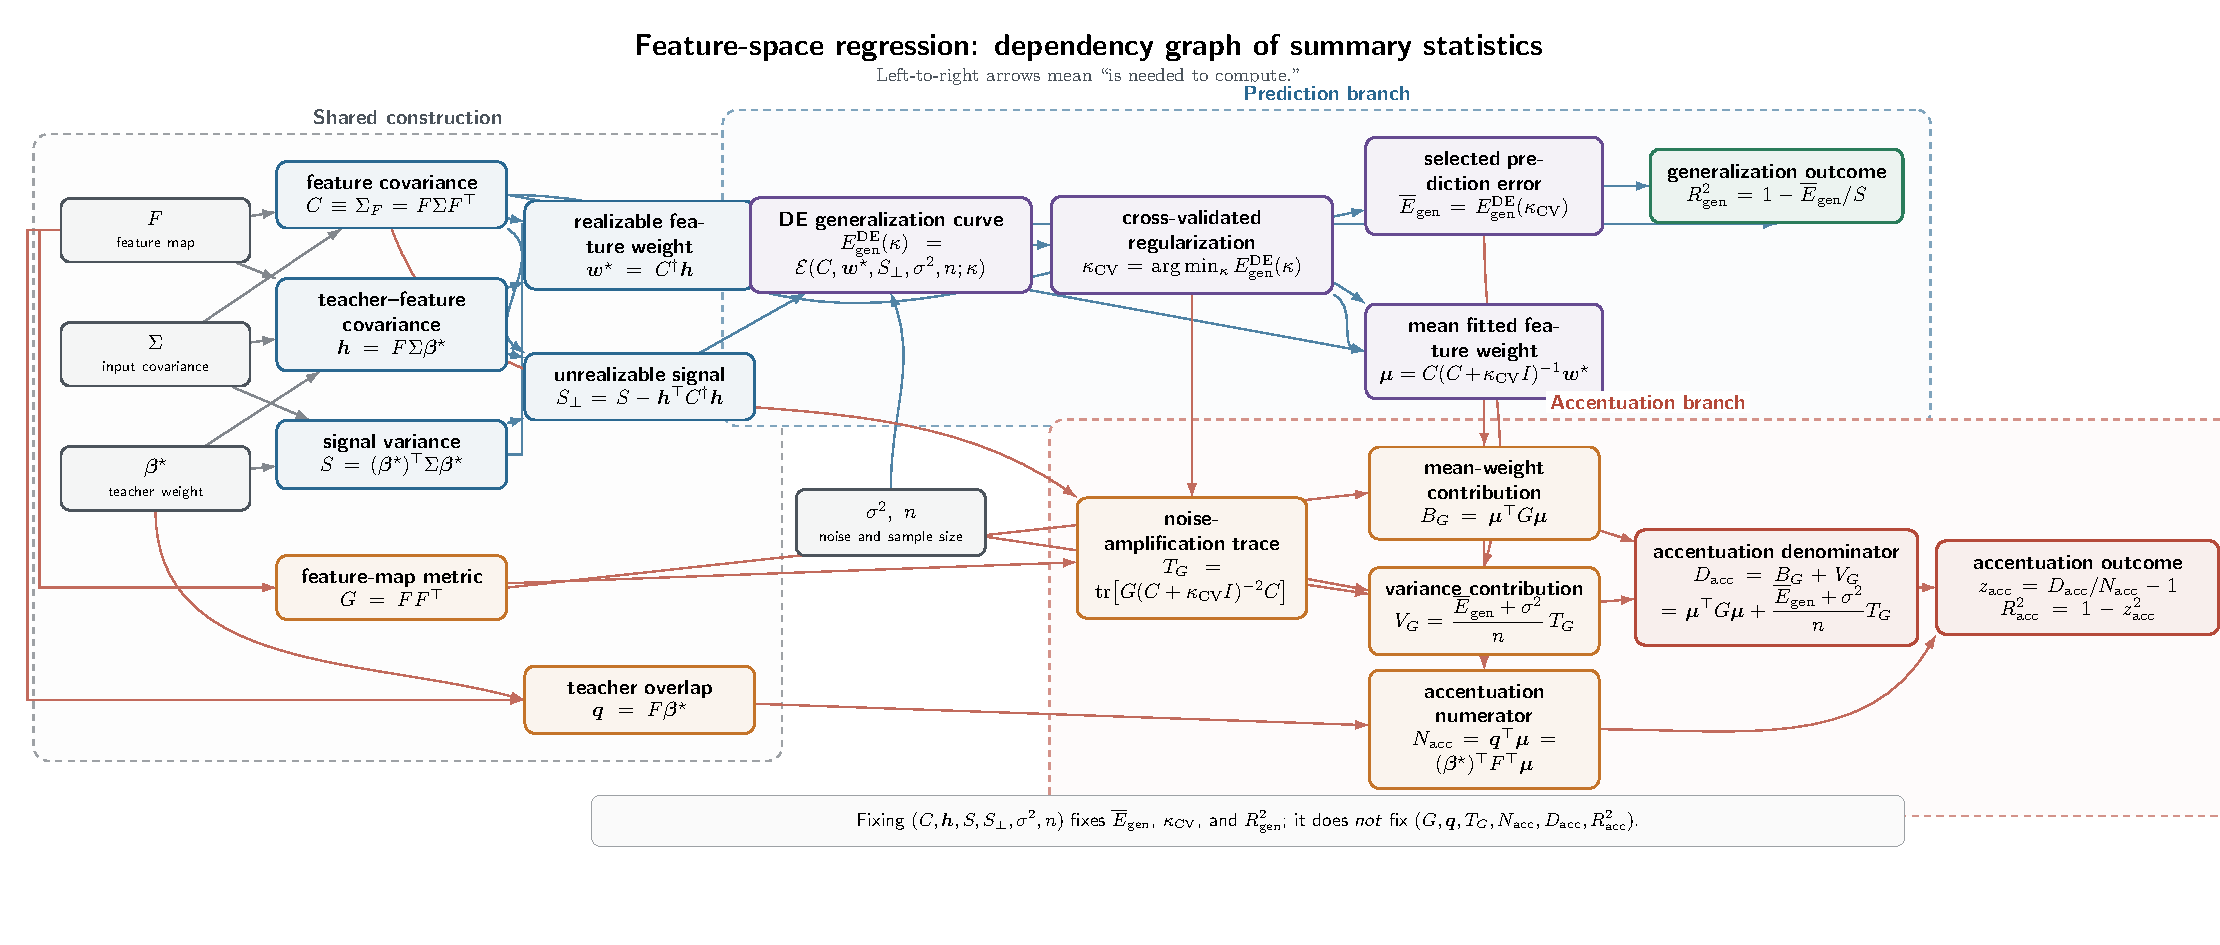
\includegraphics[width=0.55\linewidth,height=0.22\textheight,keepaspectratio]{figures/feature_summary_statistics_flow.pdf}%\hfill
    % 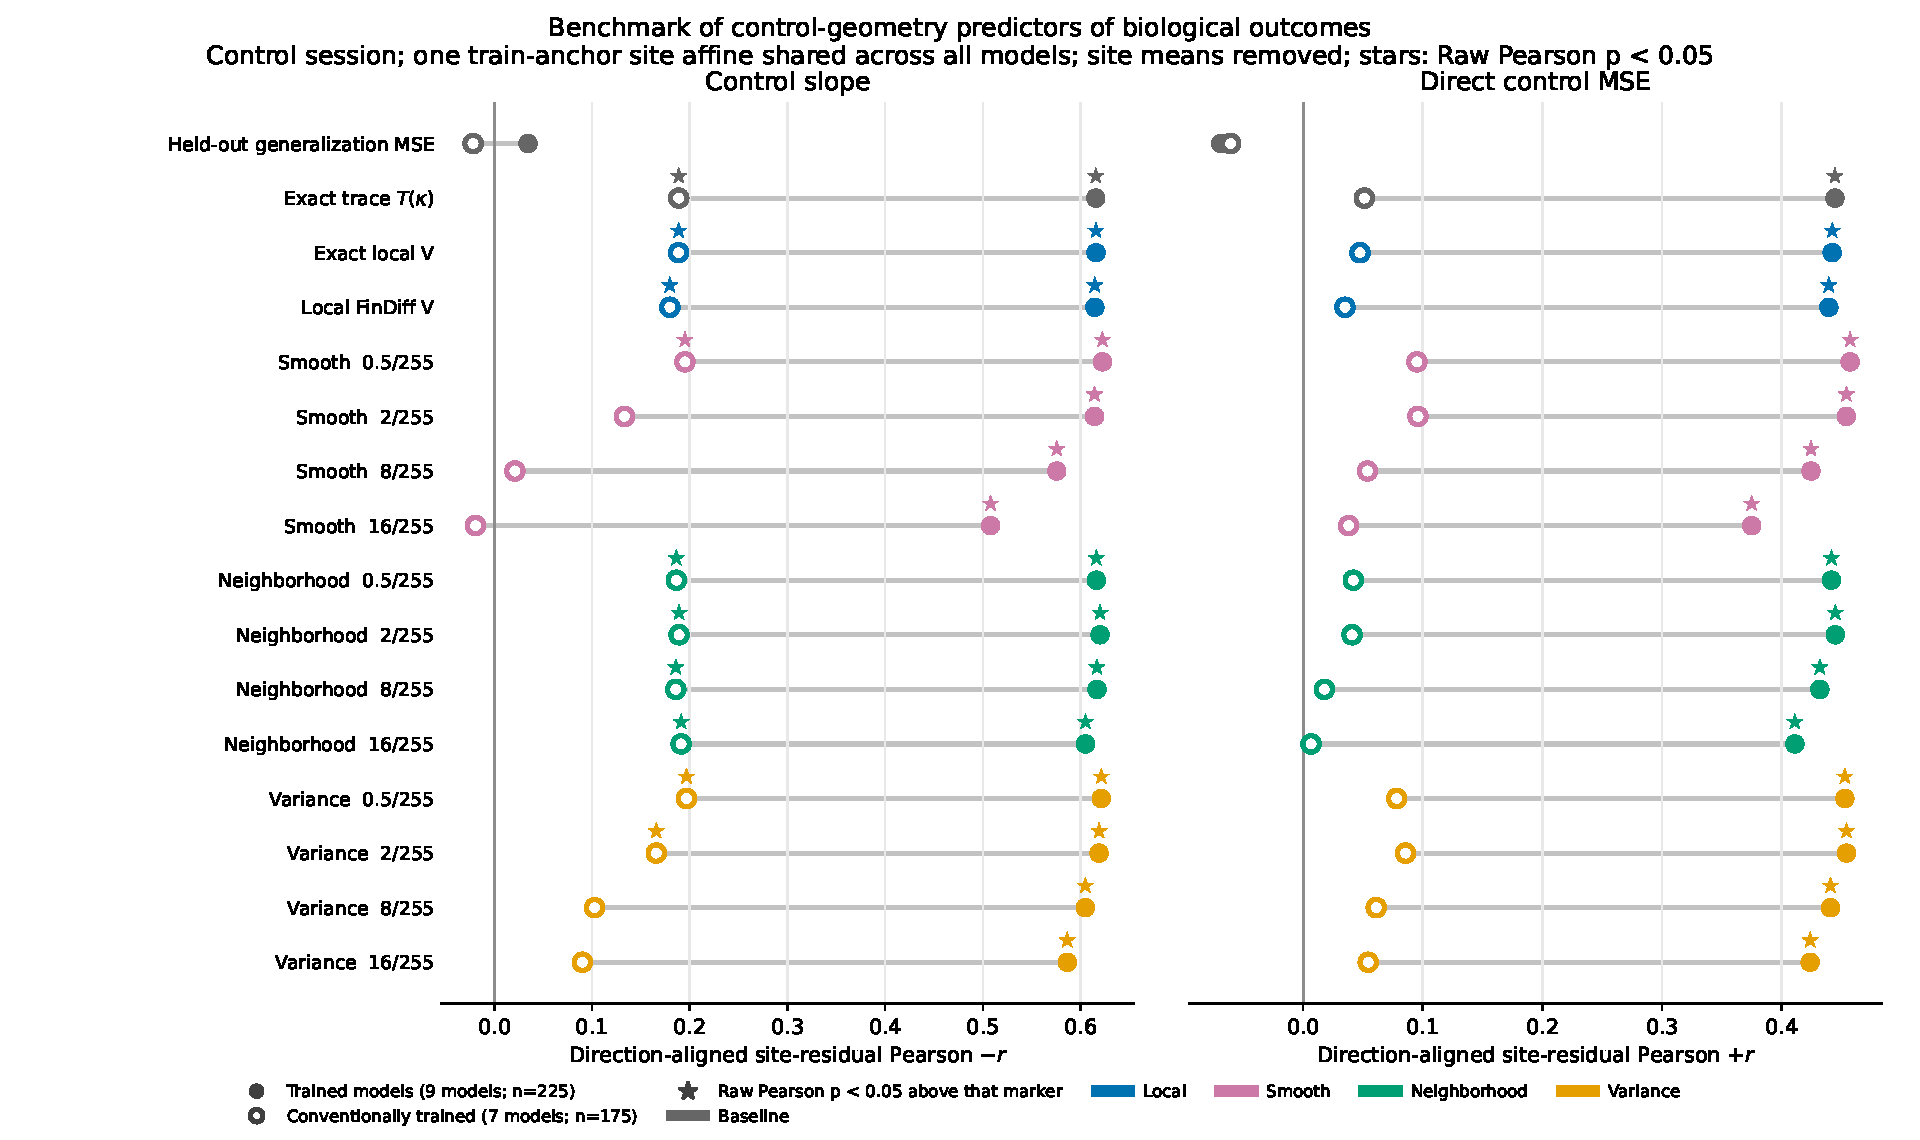
\includegraphics[width=0.44\linewidth,height=0.22\textheight,keepaspectratio]{figures/nonlinear_control_biological_validation.pdf}\\[2pt]
    % 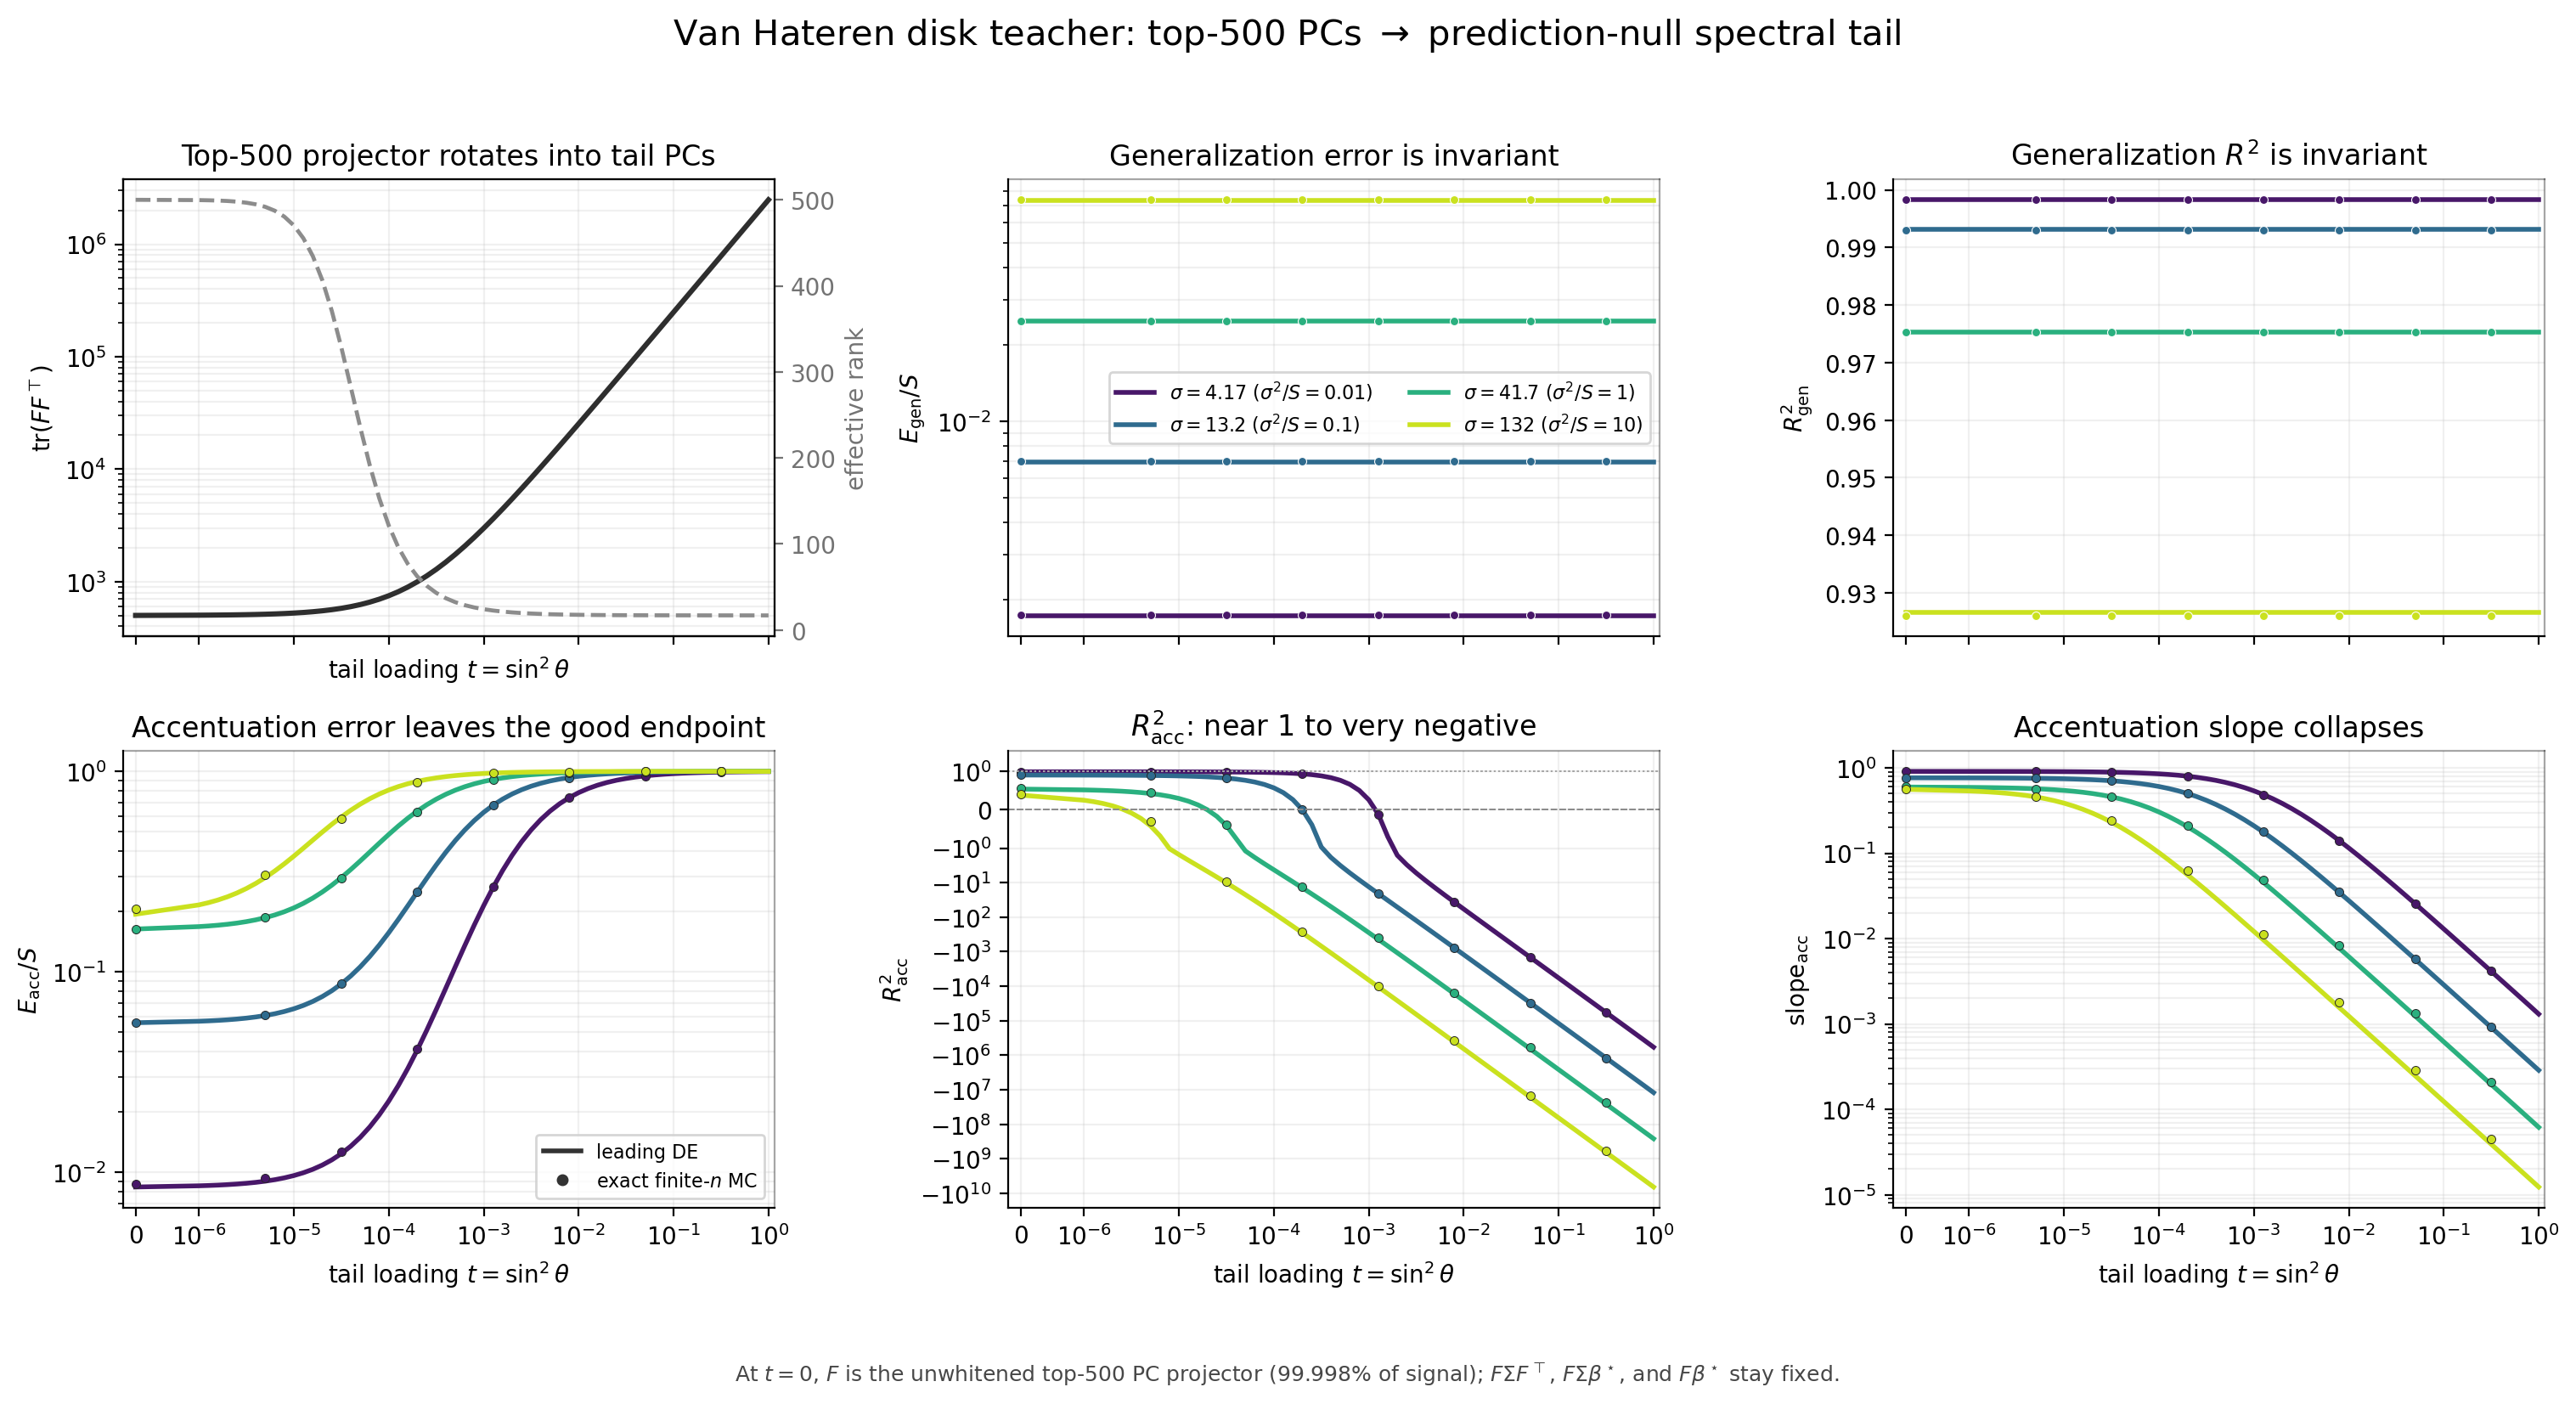
\includegraphics[width=0.45\linewidth,height=0.2\textheight,keepaspectratio]{figures/VanHateren_Top500PC_prediction_null_feature_rotation.png}
    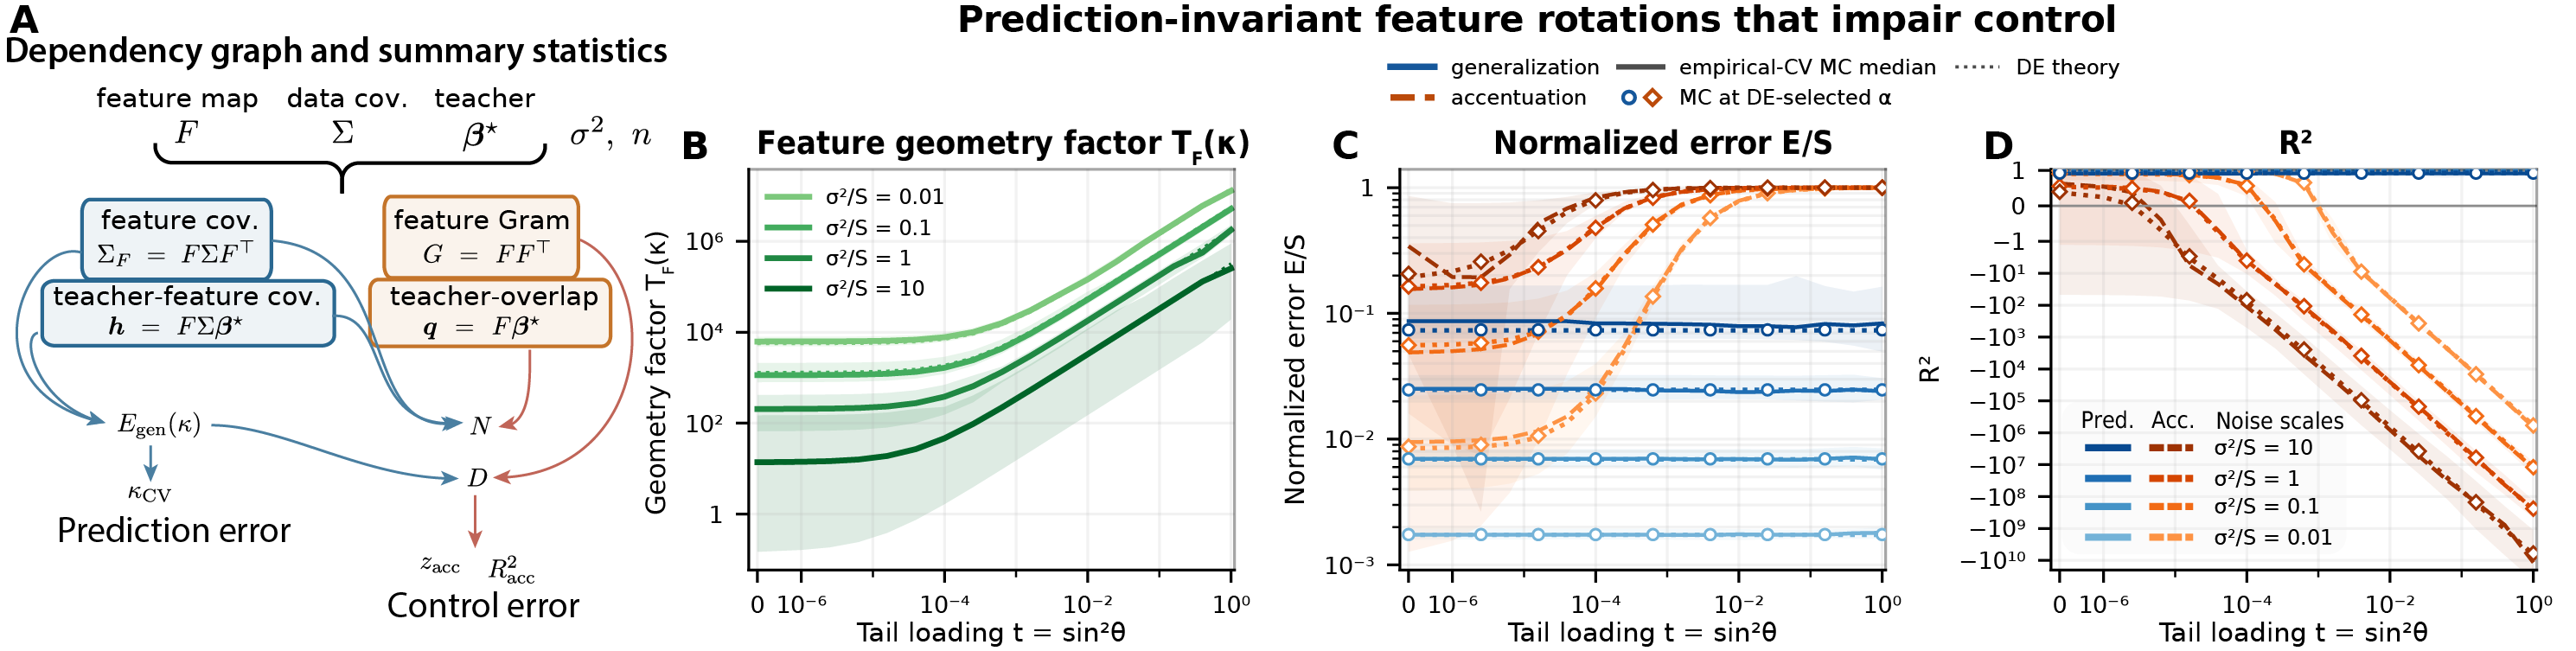
\includegraphics[width=\linewidth]{figures/Figure_linear_feature_gauge.png}
    \vspace{-15pt}
    \caption{\textbf{Feature geometry decides control.}
    \textbf{A}~Dependency graph: $(\Sigma_F,F\Sigma\bstar,S,\sigma^2,n)$ fix generalization and the cross-validated penalty; control additionally needs $\GramDef$ and $F\bstar$ (full graph: Fig.~\ref{fig:summary_stats_dep_graph}). 
    \textbf{B-D}~For van Hateren images, rotating the top-500-PC projector feature into the spectral tail: $E_{gen}$ and $R^2_{gen}$ are invariant while $R^2_{acc}$ and the slope collapse; DE (lines) matches finite-$n$ Monte Carlo (markers). Construction: App.~\ref{sec:app-methods-feature}; further rotations: App.~\ref{sec:app-ext-gauge}. }
    %\textbf{C}~Neuronal data: site-demeaned association of each candidate predictor with biological control slope (left) and control error (right) across nine trained (filled) and seven conventionally trained (open) models. Held-out error carries no model-order information; the exact trace, $V_\phi$ and its neighborhood versions do. (Draft: keep 5 rows.)}
    \label{fig:feature}%\label{fig:nonlinear-biological-validation}
\end{figure}

\section{Linear feature ridge: the map decides what reaches the gradient}
\label{sec:feature}

Pixel regression explains why one student fails; it cannot explain why ten equally predictive backbones fail differently. We idealize a backbone as a fixed linear map $F\in\R^{p\times d}$, fit $\hat w$ by ridge on features $F\x$, and accentuate along the pixel gradient $\bhat=F^\top\hat w$. Let $\Sigma_F:=F\Sigma F^\top$ be the feature covariance and $\GramDef$ the Euclidean feature Gram. The best realizable feature weight and its irreducible error are $w^\star=\Sigma_F^\dagger F\Sigma\bstar$ and $S_\perp=S-{w^\star}^\top \Sigma_F w^\star$ (App.~\ref{lem:mr-feature-weights}).

\begin{prop}[Feature ridge: prediction and control]\label{prop:feature-de}\label{prop:linfeat_acc_ND}\label{prop:linfeat_gen_err}
With $\kappa$, $B^F$ and $\mathrm{df}^F$ built from $(\Sigma_F,w^\star)$ and aspect ratio $p/n$, the mean fitted pixel weight is the realizable weight shrunk in feature space and back-projected, and the norm inflation carries a map-dependent \emph{gradient-geometry factor} $T_F$:
\begin{gather}
\bar\beta_{F,\kappa}:=F^\top(\Sigma_F+\kappa I)^{-1}F\Sigma\bstar,\quad
V_F(\kappa):=\frac{E_{gen,DE}+\sigma^2}{n}\,T_F(\kappa),\quad
T_F(\kappa):=\operatorname{Tr}\big[\Gram(\Sigma_F+\kappa I)^{-2}\Sigma_F\big],
\label{eq:feature-mean-variance}\\
E_{gen,DE}=\frac{n(\kappa^2B^F_{1,2}+S_\perp+\sigma^2)}{n-\mathrm{df}^F_2}-\sigma^2,\qquad
N_{DE}={\bstar}^\top\bar\beta_{F,\kappa},\qquad
D_{DE}=\|\bar\beta_{F,\kappa}\|^2+V_F(\kappa).
\label{eq:feature-de}
\end{gather}
Setting $F=I$ gives $\bar\beta_{F,\kappa}=\bar\beta_\kappa$ and $T_F=\mathrm{df}_{1,2}$, recovering Prop.~\ref{prop:pixel-de}. (Proofs: App.~\ref{sec:app-feature-regression}.)
\end{prop}
The structure is the same as in pixel ridge, so the reading carries over: $N$ is the teacher's alignment with the mean weight, $D$ is that weight's norm plus an inflation, and the unrealizable signal $S_\perp$ simply acts as extra response noise. What changes is what determines the two objects. Prediction sees the feature map only through $\Sigma_F$ and $F\Sigma\bstar$: the whole curve $E_{gen,DE}(\kappa)$, hence the cross-validated $\kappa$ and $R^2_{gen}$, is a function of $(\Sigma_F,F\Sigma\bstar,S,\sigma^2,n)$. Control additionally depends on the Gram $\Gram$, through $T_F$ and $\|\bar\beta_{F,\kappa}\|$, and on the teacher overlap $F\bstar$, through $N_{DE}$ (Fig.~\ref{fig:feature}A; Cor.~\ref{cor:mr-summary-statistics}). Thus the statistics governing control generically exceed those governing prediction. They coincide only in special cases, for instance white data $\Sigma=I$, where $\Gram=\Sigma_F$ and $F\bstar=F\Sigma\bstar$ (App.~\ref{sec:app-gauge-fragility}).
This extra freedom is exposed by the group of map transformations that leave prediction unchanged. 
\begin{prop}[Prediction-preserving gauge]\label{prop:gauge}
For $\Sigma\succ0$ and any orthogonal $Q$ with $Q\Sigma^{1/2}\bstar=\Sigma^{1/2}\bstar$, the map $F\mapsto F\Sigma^{1/2}Q\Sigma^{-1/2}$ preserves $\Sigma_F$ and $F\Sigma\bstar$, hence the joint feature--response covariance, $E_{gen,DE}(\kappa)$ and the DE-based prediction-optimal penalty $\kappa^\star_{gen}$, while changing $\Gram$ and $F\bstar$ and therefore control (Prop.~\ref{prop:mr-gauge}; construction in App.~\ref{sec:app-gauge-fragility}).
\end{prop}
The gauge changes control only for anisotropic inputs, increasingly so with anisotropy. Rotating within it moves feature energy from high-variance to low-variance pixel directions at no cost to prediction (Fig.~\ref{fig:feature}B): along a continuous path, $E_{gen}$, $R^2_{gen}$ and the selected penalty are exactly constant, while $\operatorname{Tr}(FF^\top)$ grows by four orders of magnitude and $R^2_{acc}$ falls from near one to $-10^{8}$. 
%\red{Random draws from the \textit{rotation group} span a huge range (Fig.~\ref{fig:supp-null-random}), so a population of equally predictive backbones with widely different control is the generic situation, not a construction.}

% For white data, the accentuation error is also invariant across this gauge group, leading to no dissociation. 

\paragraph{What makes a map fragile.}
The response-independent part of $V_F$ is the geometric factor $T_F$, which has the spectral form
\begin{equation}
T_F(\kappa)=\sum_{k:s_k>0}\Big(\frac{s_k}{s_k+\kappa}\Big)^2\frac{\|g_k\|^2}{g_k^\top\Sigma g_k},
\qquad g_k:=F^\top v_k,
\label{eq:TF}
\end{equation}
with $(s_k,v_k)$ the eigenpairs of $\Sigma_F$ (Prop.~\ref{prop:mr-fragility}). It averages, over the feature PCs that survive ridge shrinkage ($s_k^2/(s_k+\kappa)^2\sim1$), the ratio between the Euclidean energy of the backpropagated PC gradient $\|g_k\|^2$ and its energy under the natural-image covariance $g_k^\top\Sigma g_k$. Thus, a map is fragile when its \textit{well-resolved feature directions backpropagate into low-variance, high-spatial-frequency pixel directions}. This is the linear counterpart of the third observation of Sec.~\ref{sec:phenomena}, and it can be computed from the map and the image statistics alone.

\paragraph{Summary: When is control fragile although prediction is fine?}
Holding the prediction error fixed, the leading control error (Eqs.~\ref{eq:pixel-de}, \ref{eq:pixel-zacc-cv}, \ref{eq:feature-de}) grows with three separable factors:
\textbf{(i) noise} $(E_{gen}+\sigma^2)/n$, the estimation-noise level, which is the only factor visible from held-out accuracy;
\textbf{(ii) spectrum} the mismatch between prediction-optimal and control-optimal penalties, Eq.~\ref{eq:pixel-zacc-cv}, which is zero for white data and grows with anisotropy and with teacher energy in low-variance modes;
\textbf{(iii) map} $T_F$, the ridge-weighted ratio of Euclidean to natural-covariance gradient energy, a property of the feature map alone.
Noisy neuronal responses \red{\cite{?}} supply (i), natural images make (ii) large for every model, and the feature map decides (iii), in which equally predictive maps can differ without bound.



\begin{figure}[t]
    \centering
    \vspace{-15pt}
    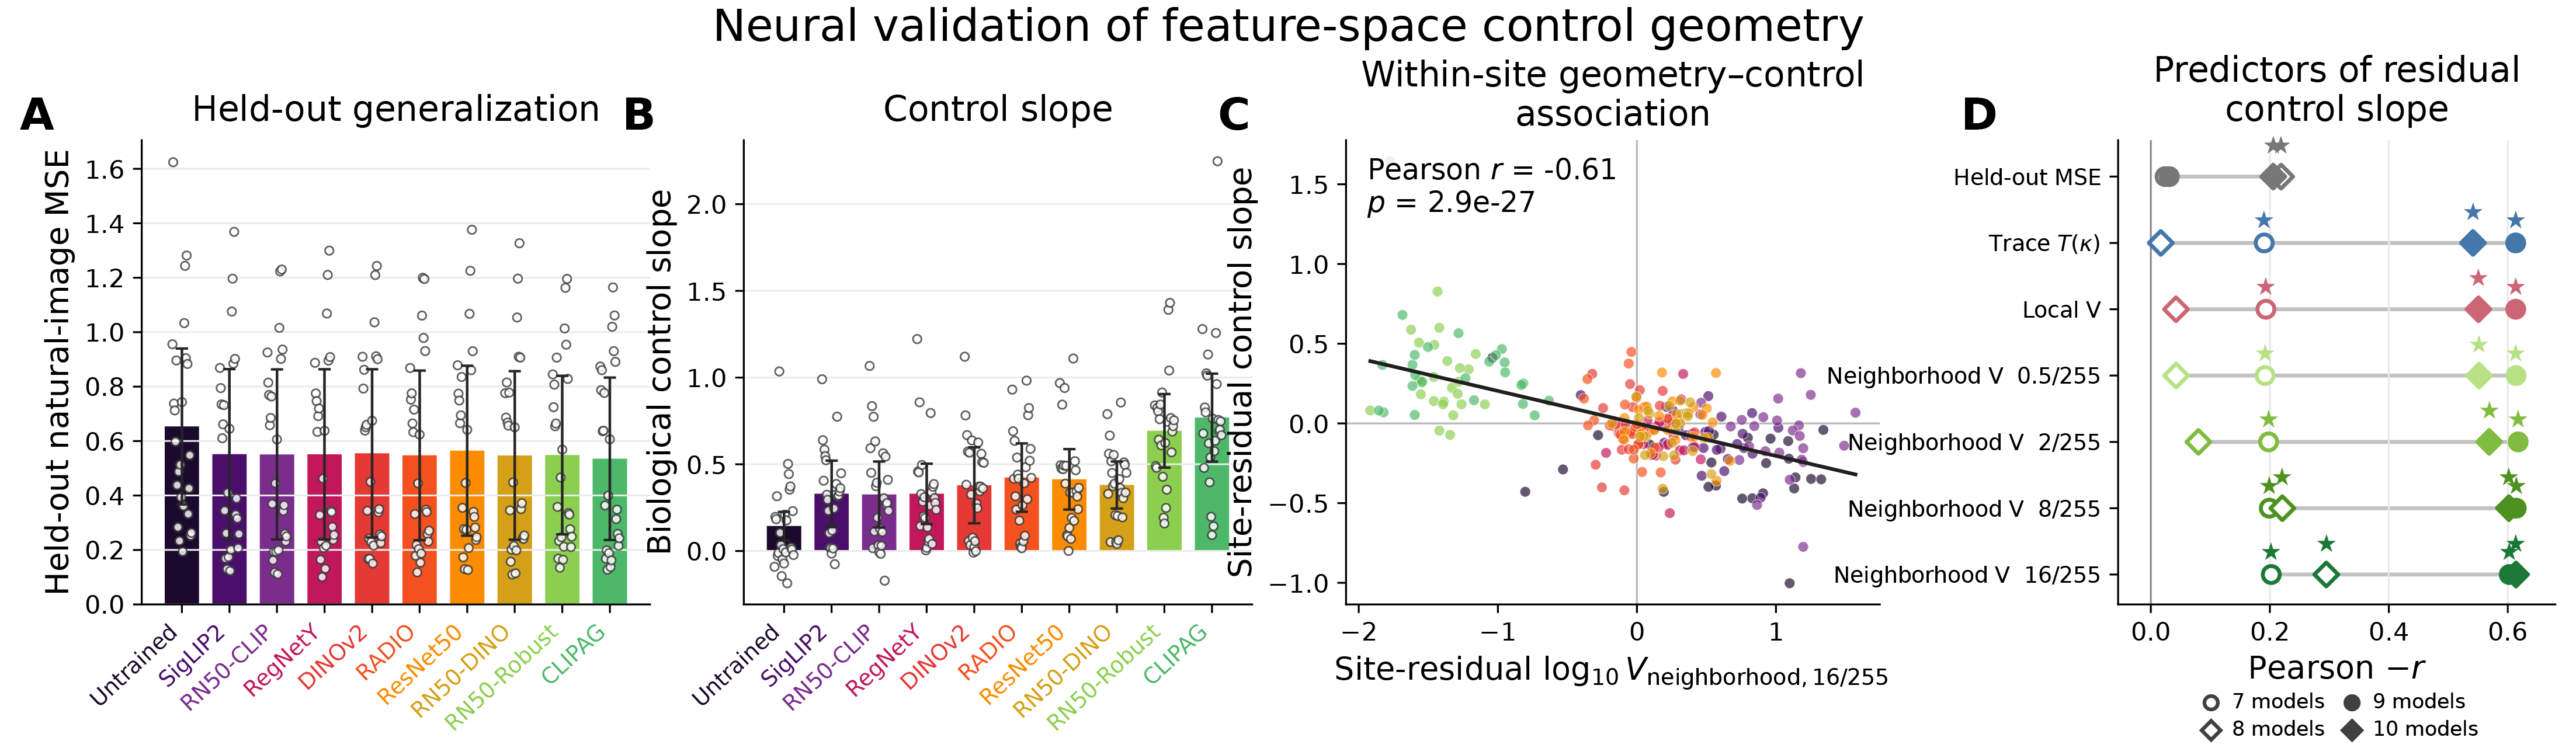
\includegraphics[width=\linewidth]{figures/Figure_nonlinear_neuro_diagnostic.png}
    \vspace{-18pt}
    \caption{\textbf{Nonlinear gradient-feature geometry predicts biological control across encoding models.}
% We evaluated ten encoding models at 25 neural recording sites from five subjects. Control-session responses were aligned to the encoding-session scale using a site-specific affine map fitted only on repeated natural-image anchors and shared across models.
Published preprocessed data of \citetPW.
\textbf{A}~Held-out natural-image MSE in the control session ($E_{\mathrm{val}}\approx E_{\mathrm{gen}}+\sigma^2$).
\textbf{B}~Slope of measured on predicted responses to accentuated stimuli. \textbf{A,B}: mean over 25 sites (bars), sites (dots), $\pm1$ SE.
\textbf{C}~Raw $\log_{10}V_\phi$ ($16/255$ neighborhood) against control slope with each site's ten-model mean removed (Pearson $r=-0.56$, 250 site--model pairs).
\textbf{D}~Pearson $-r$ between site-centered control slope and seven raw $\log_{10}$ predictors (held-out MSE, $T_\phi(\kappa)$, exact-local and neighborhood $V_\phi$ at four scales) for 10/9/8/7-model subsets (all / no untrained AlexNet / no robust models / neither); stars: raw two-sided $p<0.05$. All estimators: App.~\ref{sec:app-ext-nonlinear}.} %without multiple-comparison correction
    \label{fig:nonlinear-biological-validation}
\end{figure}

\section{Nonlinear feature ridge: a generalized diagnostic for deep networks}
\label{sec:nonlinear}
For a nonlinear feature map $\phi$ with Jacobian $J_\phi(x)$ and natural-image feature covariance eigenpairs $(s_k,v_k)$, replacing $F$ by the local Jacobian in Eq.~\ref{eq:TF} gives
\begin{equation}
T_\phi(x,\kappa)=\sum_k\frac{s_k}{(s_k+\kappa)^2}\,\|J_\phi(x)^\top v_k\|^2,
\qquad
V_\phi:=\frac{E_{val}}{n}\,\E_x\big[T_\phi(x,\kappa)\big],
\label{eq:Tphi}
\end{equation}
where $J_\phi(x)^\top v_k=\nabla_x[v_k^\top\phi(x)]$ is the pixel gradient of feature PC $k$, obtainable by one backward pass per PC, and $V_\phi$ mirrors the norm inflation $V_F$ of Eq.~\ref{eq:feature-mean-variance} with $E_{val}\approx E_{gen}+\sigma^2$. It is exact for linear $\phi$ and a theory-motivated diagnostic for networks, where $s_k=g_k^\top\Sigma g_k$ no longer holds. Since an accentuation path travels far from the seed, we also average the Jacobian, or the squared gradient, over a Gaussian neighborhood of the seed at pixel-noise scales $0.5$--$16/255$ (App.~\ref{sec:app-nonlinear-diagnostic}).

We computed these quantities for all 250 site--model pairs of the neuronal experiment (App.~\ref{sec:app-methods-nonlinear}), using each model's cross-validated ridge penalty and empirical feature spectrum to set $\kappa$, the ten experimental seed images for $\E_x$, and the held-out natural-image error of the control session for $E_{val}$. Because sites differ greatly in how controllable they are at all, we compare predictors after removing site means, so that each predictor is judged on ordering the ten models within a site (Fig.~\ref{fig:nonlinear-biological-validation}). Held-out prediction error carries essentially no information about which model will control better: its site-residual correlation with control slope is $0.03$ and with direct control error $-0.07$. The exact-local $V_\phi$ reaches $0.62$ with control slope and $0.44$ with control error across the nine trained models, and the trace $T_\phi$ alone does nearly as well, so the ordering comes from gradient geometry rather than from the prediction-error prefactor. Among the seven conventionally trained models the association is weaker but same-signed ($\approx0.2$ with slope), consistent with the two adversarially trained models being the strongest controllers and having by far the smallest $T_\phi$. Neighborhood-smoothed versions preserve or slightly improve the ordering.


\section{Discussion}
\label{sec:discussion}
A single mechanism accounts for the three neuronal phenomena: prediction measures weight error in the covariance metric, control measures it along the model's own gradient. In the linear theory the control error at fixed prediction error is governed by the three factors of the box in Sec.~\ref{sec:feature}: noise, spectrum, and map, of which only the first is visible from held-out accuracy. The practical implication is that selecting encoding models or penalties by held-out prediction cannot certify gradient-based control; validation must constrain the gradient, for instance through $T_\phi$, or test generated stimuli directly. The high-frequency artifacts of failed accentuations are not a cosmetic defect but the expected signature of low-variance directions that natural images never constrained.

\paragraph{Limitations.}
The theory assumes Gaussian inputs, a linear teacher, a fixed linear feature map and a one-dimensional accentuation path from a centered seed; the leading DEs predict typical fits and the location of the control optimum but not the fluctuation-dominated error at that optimum (App.~\ref{sec:app-ratio-corrections}). The nonlinear diagnostic is not a theorem; its biological validation is descriptive (repeated models within sites) and concerns model ordering, not absolute control error. Extending the DEs to learned nonlinear features and curved accentuation paths is the natural next step.
